\documentclass[12pt]{article}
\usepackage{authblk,pgfplots,tabularx}
\pgfplotsset{compat=1.18}
\usepackage{xurl}
\usepackage{hyperref}
% Packages for math
\usepackage{amsthm, amssymb,amsfonts}

\usepackage{physics} % Clean vector, derivative, norm, etc.

% Graphics and tables
\usepackage{graphicx}
\usepackage{float} % Improved float handling
\usepackage{booktabs} % Nicer tables
\usepackage{lscape}
\usepackage{pdflscape}
\usepackage{framed}
\usepackage{pifont}
\usepackage{array}
\usepackage{enumitem}
\usepackage[most]{tcolorbox}

\providecommand{\RR}{\mathbb{R}}




% ============================
% Complexity class and WCC macro definitions
% ============================
\renewcommand{\P}{\mathbf{P}}
\newcommand{\NP}{\mathbf{NP}}

\newcommand{\PWCC}{\mathbf{PWCC}}
\newcommand{\NPWCC}{\mathbf{NPWCC}}
\newcommand{\phys}{\mathrm{phys}}


% ============================
% Machine model macros
% ============================
\newcommand{\TM}{\mathrm{TM}}
\newcommand{\WCC}{\mathrm{WCC}}

% ============================
% Encoding / decoding macros
% ============================
\newcommand{\enc}{\mathrm{enc}}
\newcommand{\dec}{\mathrm{dec}}

% ============================
% NC hierarchy (small caps)
% ============================
\newcommand{\NC}{\mathsf{NC}}

% ============================
% Misc formatting
% ============================
\newcommand{\SAT}{\mathrm{SAT}}





\usepackage{tikz}
\usetikzlibrary{arrows.meta, positioning}

% Hyperlinks
\usepackage{hyperref}
\usepackage{tcolorbox} 

% Optional: define styling once
\tcbset{
  highlight theorem/.style={
    colback=blue!5!white,
    colframe=blue!75!black,
    fonttitle=\bfseries,
    coltitle=black,
    boxrule=0.8pt,
    arc=3pt,
    title={\textbf{Classical Implication Template: $P$ vs.\ $NP$ (Conditional)}},
    before upper={\parindent15pt},
  }
}

\title{P vs NP in Curvature-Bounded Wave Computation\\
A Model-Relative Separation Program and Corrected Proof Obligations}


\author{Richard J. Reyes}
\date{Revised October 27, 2026 \\ \small Original Release: May 7, 2025}

\theoremstyle{remark}
\newtheorem*{remark}{Remark}
\newtheorem{theorem}{Theorem}[section]
\newtheorem{lemma}[theorem]{Lemma}
\newtheorem{corollary}[theorem]{Corollary}
\newtheorem{definition}[theorem]{Definition}
\newtheorem{proposition}[theorem]{Proposition}
\newtheorem{conjecture}[theorem]{Conjecture}
\newtheorem{hypothesis}{Hypothesis}[section]
\begin{document}
\maketitle
\begin{abstract}
We study curvature-regulated wave computation (WCC) as a possible
physical resource model for decision and verification problems. We
distinguish the \emph{uniform discrete} finite-state WCC abstraction from
WCT implementations additionally constrained by curvature, field
regularity, precision, and physical energy rails. Under polynomial-time
uniform encodings and readouts, the discrete WCC model simulates and is
simulated by classical Turing machines with polynomial overhead, as
developed separately in \emph{Discrete Wave-Constrained Computation and
Classical Complexity}. This equivalence alone proves no equivalence of
physical curvature costs.

We correct the Boolean phase encoding of $3$-SAT: a signed literal score
and a product-of-unsatisfied-literals clause penalty give an exact
zero-penalty characterization of SAT assignments. This is a logical
encoding theorem, not a proof that a satisfying assignment is a stationary
point of the full WCT functional. We also exhibit a smooth finite-energy
four-dimensional field, refuting an earlier inference from failure of a
Sobolev embedding to universal infinite curvature energy.

The proposed locked-expander curvature lower bound
$C_\Theta(F_n)\ge 2^{\Omega(n)}$ is stated as a \emph{conditional research
hypothesis}: expansion alone does not establish an exponential area
lower bound for every physical encoding, and a cost of enumerating
clause-signature sectors does not bound all decision algorithms. A
conditional separation of physical WCC classes would require a genuine
language-level lower bound against every admissible deterministic
decider, along with a physically admissible polynomial-resource verifier.
The classical $\mathbf{P}$ versus $\mathbf{NP}$ problem is not resolved.

This revision records explicit mathematical counterexamples and precise
remaining obligations under tags \texttt{WIN-01}--\texttt{WIN-08}.
\end{abstract}

\section*{Current Lean formalization status (7 November 2026)}
\addcontentsline{toc}{section}{Current Lean formalization status}
\label{sec:current-lean-status}
The amended Part I manuscript has 41 inventory claims:
30 Exact under their stated hypotheses, one Restricted,
four Refuted, and six Open.  Exact includes
\emph{proved conditional implications} and does
not certify their antecedents or a solution to
classical $\mathbf P$ versus $\mathbf{NP}$.
The four false state-to-language inferences
(I-25 through I-28) have been explicitly withdrawn
in the revised sections below.  Their Lean
counterexamples remain in the historical audit.
The Restricted item I-11 concerns the missing
resource-preserving \emph{physical} WCC bridge;
the Open claims I-2, I-3, I-16, I-31, I-32
and I-37 require additional independent theorems.

\paragraph{Exact discrete model and scope.}
The repository formalizes
$P_{\mathrm{WCC}}^{\mathrm{disc}}=P_{\mathrm{TM}}$
and $NP_{\mathrm{WCC}}^{\mathrm{disc}}=NP_{\mathrm{TM}}$
for its explicitly defined finite-state models,
including the uniform version that charges
lattice generation, input encoding and readout
(\nolinkurl{PartIIUniform.P_disc_eq_P_TM},
\nolinkurl{PartIIUniform.NP_disc_eq_NP_TM}).
The older fixed-radius, origin-marked
one-dimensional models and higher-dimensional
sweep simulations have separate verified
equivalences in \texttt{PVNP.Discrete}.
The original two-phase machine $W_M$ still
needs proofs that its \emph{complete original}
lattice and input-state writers run in
polynomial single-tape time (Part II II-10).
Generic class equivalence does not complete
that particular construction.
\emph{Addendum, 12 November 2026:} both writer
proofs now exist in Lean
(\nolinkurl{TwoPhasePolynomialWriter.originalWindowCode_fp},
\nolinkurl{TwoPhasePolynomialWriter.originalInputCode_fp}),
and II-10 is Exact.

\paragraph{What the SAT and curvature results establish.}
The $\psi$-SAT logical penalty
characterizes Boolean satisfiability under
the stipulated field representation.
A logical-energy value strictly below $1/8$
supplies a formula-dependent SAT certificate;
it does not construct the phase field or
prove convergence of a physical PDE.
The classical discrete Cook--Levin reduction
and the restricted crossing-sequence
single-tape SAT lower bounds are supporting
formal results, but do not yield
$\mathrm{SAT}_{\mathrm{dense}}\notin P_{\mathrm{TM}}$.
The uniform separator-price, physical
expander hardness and construction
lower-bound premises remain Open.
Exact finite symbol counts and stable sign
encoding likewise do not yield decision
lower bounds when decoder cost is unconstrained.

\paragraph{Physical and numerical boundary.}
The repository has scoped analytic and
Lean results for frozen cubic--quintic
field equations, including a separate
$H^2$ periodic-torus well-posedness
formalization in Phase VI, stated under
its fixed equation and parameter hypotheses.
The particular preparation, precision,
detector and evolution cost required for
a universal physical SAT lower bound
have not been established.  Finite-grid
numerical overlap observations are
empirical and cannot be generalized
to all polynomial-time deciders.

\paragraph{Verification provenance.}
The old October and early-November
partial-status assertions are preserved
in the version history and claim ledger,
but are not current statements.
Some Phase XII and XIII sources were
merged while hosted Actions jobs
failed \emph{before executing any steps}.
A fresh exact-head full Lean kernel
build and standard-axiom audit are
required before newly added declarations
are described as independently verified.
A successful PDF build is separate
from this mathematical check.

\section{Introduction}
The $\mathbf{P}$ vs.\ $\mathbf{NP}$ problem asks whether every computational problem
whose solution can be verified in polynomial time can also be solved in
polynomial time. Despite decades of effort, no proof resolving
$\mathbf{P} \stackrel{?}{=} \mathbf{NP}$ has been universally accepted.
The present work does not claim to resolve this classical question; instead,
it develops a curvature-regulated model of computation and isolates
the hypotheses necessary for a model-relative lower bound and an internal
separation program.

We work within Wave Confinement Theory (WCT), where computation is defined as
the physical or symbolic evolution of confined oscillatory systems under
curvature feedback. In this setting, stable coherent wave states play the
role of solutions, and the feasibility of reaching them under bounded
evolution defines a notion of computational difficulty.

We introduce a discrete curvature-regulated computation model (WCC) and
define complexity classes $\mathbf{P}_{\mathrm{WCC}}$ and $\mathbf{NP}_{\mathrm{WCC}}$ by
imposing polynomial bounds on evolution time and curvature/entropy budgets.
Within this model we pursue two complementary tracks:

\begin{itemize}
  \item \textbf{Analytic curvature lower bound.}
        We define a semantic curvature complexity measure $\mathbf{C}_\Theta(f)$
        based on the WCT curvature operator and show that, for a locked
        expander family of 3-SAT instances inside the WCT curvature machine,
        an exponential cost has been proposed,
        $\mathbf{C}_\Theta(F_n) \ge 2^{\Omega(n)}$.
        The interface-energy and universal-encoding hypotheses required
        for this bound are not established here. It remains an open
        mathematical objective, not a proved lower bound.

  \item \textbf{Symbolic complexity and separation program.}
        We construct a verifier for wave-coherence predicates in $\mathrm{NC}^1$,
        encode SAT instances as symbolic wave-interference constraints
        (a Cook--Levin style reduction into WCC), and formalize WCC-level
        complexity classes $\mathbf{P}_{\mathrm{WCC}}$ and $\mathbf{NP}_{\mathrm{WCC}}$.
        We then formulate a \emph{model-internal separation program}:
        under explicit geometric and dynamical hypotheses (existence of
        curvature-locked states that are verifiable but not reachable within
        polynomially many curvature-bounded WCC updates), one would obtain an
        internal separation
        $\mathbf{P}_{\mathrm{WCC}} \neq \mathbf{NP}_{\mathrm{WCC}}$.
        In this manuscript these hypotheses are stated as conjectures rather
        than claimed theorems.
\end{itemize}

Finally, we outline a conditional bridge to classical complexity.
If WCC computations and deterministic Turing computations simulate each
other with only polynomial overhead, then the WCC classes would satisfy
$\mathbf{P}_{\mathrm{WCC}} = \mathbf{P}$ and $\mathbf{NP}_{\mathrm{WCC}} = \mathbf{NP}$.
Under this \emph{TM--WCC compatibility conjecture}, any internal separation
$\mathbf{P}_{\mathrm{WCC}} \neq \mathbf{NP}_{\mathrm{WCC}}$, combined with the curvature
lower bound described above, would imply the classical separation
$\mathbf{P} \neq \mathbf{NP}$.
The specified frozen one-dimensional radius-one discrete model has a
kernel-checked polynomial-time TM/WCC equivalence. Its physical
curvature-preserving realization and any internal physical separation are
unproved. We focus on the exact logical encoding and explicit hypotheses
needed for a future model-relative analytic curvature lower bound.










\clearpage
\section*{Author's Note: On the Geometry of Computation and the Dimensional Lock}

This work proposes a new approach to the \textbf{P vs.\ NP} problem, one that
is not purely combinatorial or symbolic, but instead \emph{geometric},
\emph{topological}, and \emph{physical}. Computation here is modeled not as an
abstract string-manipulation process, but as the evolution of a wavefunction
constrained by curvature, entropy, and dimension.

The central mechanism is what I term a \textbf{dimensional lock}: in the
curvature-regulated model, attempting to force a deterministic, uniformly
controlled evolution (the analogue of $\mathbf{P}$) to realize certain
non-uniform, combinatorially large configurations (the analogue of
$\mathbf{NP}$) appears to require crossing a geometric barrier that is
forbidden by the curvature and dimensionality constraints.
At an intuitive level, this structural obstruction prevents uniform
computation from accessing the full non-uniform solution space and motivates
an internal separation
\[
\mathbf{P}_{\mathrm{WCC}} \;\neq\; \mathbf{NP}_{\mathrm{WCC}}
\]
\emph{within the WCC model}.

In the body of the paper, this idea is made precise in two steps.
First, a semantic curvature complexity measure is introduced and an exponential
curvature lower bound is proposed as a conditional goal for locked-expander
3-SAT instances inside the WCT curvature machine. Second, a discrete symbolic
abstraction of WCC is developed, together with a verifier and a set of
explicit geometric and dynamical hypotheses which, if established, would
yield a formal internal separation $\mathbf{P}_{\mathrm{WCC}} \neq
\mathbf{NP}_{\mathrm{WCC}}$.

This perspective is simple but nontraditional. It draws from physics and
information theory, disciplines not typically employed in classical
complexity theory. For that reason, it may appear unfamiliar or even
unorthodox to some readers. The claim here is not that a physical metaphor
proves a classical complexity result, but that a curvature- and
dimension-constrained \emph{symbolic} model admits (i) a precise
conditional curvature-bound program for SAT, and (ii) a carefully stated
internal separation program.

The extrapolation to the classical statement $\mathbf{P} \neq \mathbf{NP}$ is
treated explicitly as conditional. If curvature-regulated WCC machines and
standard Turing machines are polynomially equivalent in computational power,
then the dimensional lock and curvature bounds described here would provide a
route to the classical separation. That simulation equivalence is isolated as
a distinct conjecture rather than assumed silently; this paper does not claim
to resolve the classical $\mathbf{P}$ vs.\ $\mathbf{NP}$ problem.



\section{Curvature-Confinement Formalism and a Model-Internal Separation}

We propose that a confined wavefield $\psi(x, t)$ under curvature feedback
evolves toward symbolic configurations that cannot be constructed in
polynomial time but can be verified via coherence constraints. Within the
rail-constrained WCC abstraction, this creates a natural asymmetry between
generation and verification, aligning with a prospective distinction between
$\mathbf{P}_{\mathrm{WCC}}^{\mathrm{phys}}$ and
$\mathbf{NP}_{\mathrm{WCC}}^{\mathrm{phys}}$, where the superscript
$\mathrm{phys}$ denotes photonic WCT/WCC machines subject to finite-curvature,
finite-band rails (Section~\ref{sec:dim-lock}).

\subsection{Definitions}

\textbf{Curvature-Locked State}: A wavefield $\psi^*$ is curvature-locked if
it satisfies
\begin{equation}
W_\psi = \frac{-\nabla^2 \psi}{\psi + \epsilon e^{-\alpha |\psi|^2}},
\quad \text{with } \frac{dS[\psi]}{dt} \to 0 \text{ and } \nabla W_\psi \to 0
\end{equation}
under the WCT/WCC evolution rules.

\textbf{Symbolic Configuration Set} $\mathcal{S}$: A set of discrete
symbolic regions $R_i$ where
\[
\psi(x) \approx \psi_i \quad \forall x \in R_i, \quad R_i \subseteq \mathbb{R}^n
\]
implements a finite symbolic configuration (assignment, tape content, etc.)
inside the WCC model.

\textbf{Verification Operator} $\mathcal{V}$: A polynomial-time procedure on
the WCC encoding which confirms that
\[
\mathcal{V}(\psi^*, \mathcal{S}) = \text{True} \iff
\psi^* \text{ exhibits symbolic coherence consistent with } \mathcal{S},
\]
with an implementation in $\mathrm{NC}^1$ on a classical circuit model.

\textbf{Non-Constructibility Condition (WCC)}: A curvature-locked state
$\psi^*$ is \emph{non-constructible in}
$\mathbf{P}_{\mathrm{WCC}}^{\mathrm{phys}}$ if no deterministic
polynomial-time WCC machine
$\mathcal{T}_{\mathrm{WCC}}^{\mathrm{phys}}$ (obeying WCT rails) can output
$\psi^*$ from a trivial input configuration, while a polynomial-time WCC
verification $\mathcal{V}$ remains available.

\subsection{Model-Internal Complexity Schema}

Fix a state-construction model. Write $P_{\rm st}$ for states a polynomial-time
machine produces and $NP_{\rm st}$ for states the verification predicate
accepts. In Lean these sets are \texttt{ConstructionModel.Pst} and
\nolinkurl{ConstructionModel.NPst}.

\begin{proposition}[Curvature-Confinement Complexity Schema in Physical WCC]
Let $C$ be a real-valued functional and $\psi^*$ a verifiable state.
Suppose that for each polynomial-time constructor $M$ there is a number
$B_M<C(\psi^*)$ such that $C(\phi)\le B_M$ for every state $\phi$ that
$M$ produces. Then $\psi^*\in NP_{\rm st}\setminus P_{\rm st}$.
\end{proposition}
\begin{proof}
If $M$ produced $\psi^*$, its bound would give
$C(\psi^*)\le B_M<C(\psi^*)$. Verifiability gives membership in
$NP_{\rm st}$. This proves the state-set conclusion of
\nolinkurl{PartISeparation.complexity_schema}. Deriving the cost premise
from the physical dynamics remains open.
\end{proof}

\subsection{$\psi$-SAT Encoding Scheme (WCC Rail)}

Let each Boolean clause $C_i$ in a SAT instance be mapped to a spatial clause
kernel:
\begin{equation}
\psi(x, 0) = \sum_i \chi_i(x) e^{i \phi_i},
\quad \chi_i(x) \text{ localized curvature excitation},
\end{equation}
with a prescribed WCC encoding from symbolic clauses to localized modes.

The proposed physical lock tests whether local phase gradients decay and
intensity reaches a local maximum. Its equivalence to SAT remains open (I-3).
The formula-dependent logical penalty in Section~\ref{sec:psi-sat-corrected}
has a proved witness criterion.

% ============================
% Complexity Class Definitions
% ============================

\section{Complexity Class Definitions}

\begin{definition}[Class P]
$\mathbf{P}$ is the class of decision problems solvable by a deterministic
Turing machine in polynomial time, i.e., there exists a machine $M$ and
constant $k$ such that for all inputs $x$, $M(x)$ halts in
$\mathcal{O}(|x|^k)$ steps.
\end{definition}

\begin{definition}[Class NP]
$\mathbf{NP}$ is the class of decision problems for which a proposed solution
(certificate) can be verified in polynomial time by a deterministic Turing
machine. Formally, $L \in \mathbf{NP}$ if there exists a polynomial-time
verifier $V(x, w)$ and polynomial $q$ such that
\[
x \in L \iff \exists w : |w|\le q(|x|)\ \land\ V(x, w) = 1.
\]
\end{definition}

In the WCC setting we distinguish two model-relative classes:

\begin{itemize}
  \item $\mathbf{P}_{\mathrm{WCC}}^{\mathrm{phys}}$ and
        $\mathbf{NP}_{\mathrm{WCC}}^{\mathrm{phys}}$:
        rail-constrained photonic WCC machines under WCT curvature/energy
        caps (finite universe band).
  \item $\mathbf{P}_{\mathrm{WCC}}^{\infty}$ and
        $\mathbf{NP}_{\mathrm{WCC}}^{\infty}$:
        ideal discrete WCC machines without global physical caps, suitable
        for asymptotic Turing-equivalence considerations.
\end{itemize}

The main model-internal separation conjectures below concern
$\mathbf{P}_{\mathrm{WCC}}^{\mathrm{phys}}$ and
$\mathbf{NP}_{\mathrm{WCC}}^{\mathrm{phys}}$. Implications for classical
$\mathbf{P}$ vs.\ $\mathbf{NP}$ via the ideal classes
$\mathbf{P}_{\mathrm{WCC}}^{\infty}, \mathbf{NP}_{\mathrm{WCC}}^{\infty}$
are discussed only as conditional corollaries.


\clearpage


\section{Main Model-Relative Separation Statement
\texorpdfstring{ ($\mathbf{P}_{\mathrm{WCC}}^{\mathrm{phys}} \ne
                 \mathbf{NP}_{\mathrm{WCC}}^{\mathrm{phys}}$)}
                {Main Model-Relative Separation Statement: PWCCphys != NPWCCphys}}

\label{sec:model-separation}

\begin{conjecture}[Symbolic Separation Program in Physical WCC]
Under one fixed preparation, verification and resource model, there exists
a coherent target state in $NP_{\rm st}\setminus P_{\rm st}$.
\end{conjecture}
The proposed encoding associates SAT constraints with curvature-locked
fields. This conjecture requires a verifiable target and a bound against
every permitted polynomial-time constructor of that target.
Decision hardness requires one fixed input language and a worst-case bound
for every correct decider, including those that bypass the target.
Section~\ref{sec:dim-lock} discusses the proposed geometric obstruction.

\subsection{$\psi$-SAT Encoding and Symbolic Map}

We formally define the symbolic encoding from a Boolean SAT instance into
curvature-locked wave states. Let a Boolean clause
\(C_i \in \mathrm{SAT}\) be
\[
C_i = (x_1 \lor \lnot x_2 \lor x_3).
\]
We map each clause \(C_i\) directly into a wave symbol region
\( R_i \subseteq \mathbb{R}^n \):
\[
C_i \mapsto \psi_i(x) = A_i e^{i\phi_i(x)}, \quad x \in R_i,
\]
where \(A_i\) is a localized amplitude distribution enforcing clause
locality and \(\phi_i(x)\) encodes logical states (True/False) in terms of
constructive or destructive interference.

We construct the global wavefield as a coherent superposition of all clause
wavefunctions:
\[
\psi(x) = \sum_{i}\psi_i(x).
\]
The phase-gradient and local-intensity test proposed here is an open
physical readout criterion. The uniform Cook--Levin reduction applies
to the discrete symbolic language.

\subsection{Model-Internal Symbolic Separation}

\begin{theorem}[Conditional Symbolic Separation in Physical WCC]
Fix the preceding state-construction model. If its verification predicate
accepts $\psi^*$ and every polynomial-time constructor fails to produce
$\psi^*$, then $\psi^*\in NP_{\rm st}\setminus P_{\rm st}$ and
$P_{\rm st}\ne NP_{\rm st}$.
\end{theorem}
\begin{proof}
Verification puts $\psi^*$ in $NP_{\rm st}$. Membership in $P_{\rm st}$
would supply a polynomial-time constructor producing $\psi^*$, contrary to
the second hypothesis. The two sets therefore differ on $\psi^*$.
\end{proof}

\subsection{Symbolic Turing Abstraction and Conditional Classical Corollary}

In an \emph{ideal} discrete WCC model (ignoring global WCT caps), we encode
each \( \psi[i,j] = a + ib \in \mathbb{C} \) as
a binary string on a Turing tape.

\textit{Encoding:} Each cell amplitude \( \psi[i,j] \) is represented by a
finite-precision binary code on one or more Turing tapes.

\textit{Evolution:} Polynomial-time ideal WCC updates are simulated by a
deterministic Turing machine using local symbolic gates that implement the
curvature-regulated transition rules, defining classes
$\mathbf{P}_{\mathrm{WCC}}^{\infty}, \mathbf{NP}_{\mathrm{WCC}}^{\infty}$.

\textit{Verifier:} A polynomial-time predicate on uniformly encoded pairs
$(x,w)$, with a polynomial bound on $|w|$, defines an NP language by
existential quantification over witnesses. Physical overlap and entropy
tests additionally require precision and margin estimates.

\subsection{Formal Completion (Cook--Levin Consistency and Conjectural Bridge)}

The defined finite discrete model admits the two polynomial-overhead
simulations proved in Part II. Extending the classification to a continuum
PDE requires a uniform resource-preserving simulation of preparation,
evolution and readout.

\noindent
\textbf{Conditional Classical Corollary.}
If, in addition, (i) every polynomial-time Turing machine can be simulated
by a polynomial-time \emph{ideal} WCC machine (TM $\Rightarrow$
$\mathrm{WCC}^{\infty}$ with polynomial overhead) and (ii) every
polynomial-time ideal WCC machine can be simulated by a polynomial-time
Turing machine ($\mathrm{WCC}^{\infty}$ $\Rightarrow$ TM with polynomial
overhead), then
\[
\mathbf{P}_{\mathrm{WCC}}^{\infty} = \mathbf{P}, \quad
\mathbf{NP}_{\mathrm{WCC}}^{\infty} = \mathbf{NP}.
\]
Any eventual internal separation
$\mathbf{P}_{\mathrm{WCC}}^{\infty} \neq
 \mathbf{NP}_{\mathrm{WCC}}^{\infty}$,
established by strengthening the geometric barrier program to the ideal
model, would then imply the classical separation $\mathbf{P} \neq \mathbf{NP}$.

For the defined discrete language classes the simulations are proved. The decision lower bound and the continuum correspondence remain open.






\clearpage
% ============================================================
%  WCC INTERNAL COMPLEXITY THEORY — FORMAL THEOREMS
% ============================================================

\section{Internal Complexity Structure of WCC}

We present the internal complexity hierarchy of the Wave Curvature
Computation (WCC) model.  All results in this section are strictly
model-internal and do not concern classical Turing complexity.

\subsection{Preliminaries}

Let $\Lambda \subset \mathbb{Z}^d$ be a finite lattice with $d=2$ or
$d=3$.  A WCC configuration is a field
\[
  \psi : \Lambda \to \mathbb{C}.
\]

The curvature functional is
\begin{equation}
E[\psi]
=
\sum_{i\in\Lambda}
\left(
  |\nabla\psi(i)|^2
  +
  |\Theta[\psi(i)]|^2
  +
  V_F(\psi(i))
\right),
\end{equation}
where
\[
\Theta[\psi]
=
-\frac{\Delta\psi}{\psi + \epsilon e^{-\alpha|\psi|^2}}
\]
and $V_F$ encodes logical constraints.

A WCC evolution is any sequence $\psi_0,\psi_1,\psi_2,\dots$ obeying
$r$-local update rules and satisfying
\[
E[\psi_t] < \infty \quad \forall t.
\]

% ------------------------------------------------------------
\subsection{Definition of PWCC and NPWCC}

\begin{definition}[PWCC]
The class $\mathbf{PWCC}$ consists of all decision problems solvable by
a WCC evolution in $\mathrm{poly}(n)$ update steps, where $n$ is the
instance size, with the additional constraints:
\[
E[\psi_t] < \infty, \qquad
\dim_{\mathrm{eff}}(\psi_t) \le 3
\quad\text{for all } t.
\]
Here $\dim_{\mathrm{eff}}$ denotes the effective geometric embedding
dimension (Definition~\ref{def:effective-dimension}).
\end{definition}

\begin{definition}[NPWCC]
The class $\mathbf{NPWCC}$ consists of all decision problems $F$ for
which there exists a configuration $\psi$ satisfying all constraints
(i.e.\ $E_{\mathrm{logic}}[\psi]=0$), and for which such $\psi$ can be
verified in $\mathrm{poly}(n)$ time by a WCC evolution.
\end{definition}

% ------------------------------------------------------------
\subsection{$\psi$-SAT Encoding}
\label{sec:psi-sat-corrected}
\noindent\textbf{WIN-01 and WIN-02 (corrected).}
Let $F=\bigwedge_{j=1}^m C_j$ be a $3$-CNF formula on Boolean
variables $x_1,\ldots,x_n$. On each variable region, use a nonzero
field with encoded phase $\theta_i\in\{0,\pi\}$ and set
\[
x_i=1\iff\theta_i=0,\qquad x_i=0\iff\theta_i=\pi.
\]
For a literal $\ell$, write $v(\ell)$ for its variable index and set
$\eta_\ell=+1$ for $x_{v(\ell)}$ and $\eta_\ell=-1$ for
$\neg x_{v(\ell)}$. Define its truth score by
\[
 s(\ell;\psi):=\frac{1+\eta_\ell\cos\theta_{v(\ell)}}{2}.
\]
For Boolean phases the score is exactly $1$ when the literal is true,
and exactly $0$ when it is false. For a clause
$C_j=(\ell_{j1}\lor\ell_{j2}\lor\ell_{j3})$ define
\[
 V_j(\psi):=\prod_{k=1}^3\bigl(1-s(\ell_{jk};\psi)\bigr),
 \qquad E_{\mathrm{logic}}[\psi]:=\sum_{j=1}^m V_j(\psi).
\]
The product, rather than a sum of unsatisfied literals, encodes the
Boolean \emph{OR} relation. The energy is nonnegative on all nonzero
phase encodings; no division by a vanishing field amplitude is used.

\subsection{$\psi$-SAT Logical Completeness (Corrected)}
\begin{theorem}[Exact logical zero-penalty characterization]
\label{thm:psi-sat-completeness}
For every $3$-CNF formula $F$, the following are equivalent:
\begin{enumerate}
\item $F$ has a satisfying Boolean assignment.
\item There exists a binary-phase configuration $\psi$ with
$E_{\mathrm{logic}}[\psi]=0$.
\end{enumerate}
The same existential equivalence holds if arbitrary phases are permitted
and all variable amplitudes remain nonzero. Neither equivalence asserts
stationarity of the \emph{full} WCT energy functional.
\end{theorem}
\begin{proof}
If $F$ is satisfiable, give each variable phase $0$ for true and
$\pi$ for false. In every clause some literal has score $1$, and
therefore every $V_j$ vanishes. Conversely, all $V_j$ are
nonnegative, so $E_{\mathrm{logic}}=0$ implies that every clause has
at least one literal with score $1$. Since $s(\ell)=1$ forces the
corresponding phase to be exactly $0$ or $\pi$ with the appropriate
sign, these literal truth requirements are mutually consistent across
clauses. Complete any remaining unspecified Boolean variables
arbitrarily. The resulting assignment satisfies $F$.
\end{proof}

\paragraph{Quantitative witness readout.}
Assign $x_i=1$ when $\cos\theta_i\ge0$. In any clause falsified by this
assignment each of the three factors $1-s$ is at least $1/2$. Since all
clause penalties are nonnegative, $E_{\rm logic}<1/8$ guarantees that
this one assignment satisfies every clause. Along any trajectory with
$E_{\rm logic}\to0$ this holds at every sufficiently late observation.
The strict threshold for this decoder is sharp: for the single clause
$(\neg x\vee\neg x\vee\neg x)$, the phase $\pi/2$ gives energy $1/8$
and the tie rule chooses $x=1$. Convergence of the actual dynamics
remains an independent hypothesis.

\begin{remark}[WIN-03: stationarity is a separate obligation]
The implication $E_{\mathrm{logic}}[\psi]=0\Rightarrow
\delta(E_{\mathrm{geom}}+\lambda E_{\mathrm{logic}})[\psi]=0$
is invalid without conditions on the geometric first variation,
boundary data, and admissible function space. A zero of a nonnegative
logical penalty need not be stationary for an independently varying
geometric energy. Existence of a full PDE equilibrium realizing an
assignment is therefore an open problem here.
\end{remark}

\subsection{Effective Dimension}
\begin{definition}[Effective Dimension]
\label{def:effective-dimension}
For a specified admissible representation class, let
\[
\dim_{\mathrm{eff}}(\psi):=\min\{k\in\mathbb N:
\psi\text{ has the prescribed regular encoding in }\mathbb Z^k\},
\]
when the set is nonempty. Any dimension-dependent obstruction must
also specify the encoding and ambient function spaces.
\end{definition}

\subsection{The Dimensional-Lock Claim Requires Additional Hypotheses}
\begin{proposition}[WIN-04: failure of Sobolev embedding is not infinite energy]
\label{lem:dim-lock}
For $d=4$, there exist nonzero smooth localized fields with finite
$\|\nabla\psi\|_{L^2}^2$ and finite corrected regularized curvature
energy $\|\Theta_\varepsilon[\psi]\|_{L^2}^2$, where
\[
\Theta_\varepsilon[\psi]=
-\frac{\Delta\psi\,\overline\psi}
{|\psi|^2+\varepsilon e^{-\alpha|\psi|^2}},
\qquad\varepsilon>0,\quad\alpha\ge0.
\]
Consequently the failure of an $H^1\hookrightarrow L^\infty$
embedding for $d>3$ does not prove that every higher-dimensional
configuration has infinite WCT curvature energy.
\end{proposition}
\begin{proof}
Take $\psi(x)=e^{-|x|^2}$ on $\mathbb R^4$.
Then $\nabla\psi=-2x e^{-|x|^2}$ and
$\Delta\psi=(4|x|^2-8)e^{-|x|^2}$, both square-integrable.
For this real positive field, the denominator is positive and
$|\overline\psi|/(|\psi|^2+\varepsilon e^{-\alpha|\psi|^2})$
is globally bounded: near infinity its numerator tends to zero
while the denominator tends to $\varepsilon$, and on compact
intervals of amplitudes it is continuous. Thus
$\Theta_\varepsilon[\psi]\in L^2(\mathbb R^4)$.
\end{proof}
\begin{remark}
This does not prove stability or existence of physically confined
four-dimensional solitons. It invalidates the claimed \emph{universal
infinite-energy deduction}; a dimensional obstruction requires a
separate theorem specifying its PDE, admissible states, and rails.
\end{remark}

\subsection{Internal Separation: Conditional Language-Level Statement}
\begin{proposition}[WIN-05: conditional physical-WCC separation]
\label{thm:pwcc-neq-npwcc}
Fix the same physical encoding, resource bounds, uniformity conditions,
and language definition for both
$\mathbf{P}_{\mathrm{WCC}}^{\mathrm{phys}}$ and
$\mathbf{NP}_{\mathrm{WCC}}^{\mathrm{phys}}$.
If some language $L$ has a polynomial-resource physical WCC verifier
with polynomial-size witnesses, but every physically admissible
\emph{deterministic decider} for $L$ exceeds at least one polynomial
resource rail infinitely often, then
\[
\mathbf{P}_{\mathrm{WCC}}^{\mathrm{phys}}\ne
\mathbf{NP}_{\mathrm{WCC}}^{\mathrm{phys}}.
\]
This proposition is conditional; the requisite universal lower bound
is not proved here.
\end{proposition}
\begin{proof}
The verifier hypothesis gives
$L\in\mathbf{NP}_{\mathrm{WCC}}^{\mathrm{phys}}$.
The lower-bound hypothesis gives
$L\notin\mathbf{P}_{\mathrm{WCC}}^{\mathrm{phys}}$.
Both refer to the same language and physical resource accounting, so
the classes differ.
\end{proof}

\section{Curvature collapse and loss of grammatical structure}

This subsection separates a high-curvature condition from a distinct,
testable mixing hypothesis on observable transitions. Exceeding a
curvature rail alone does not imply the loss of a finite symbolic
partition, language triviality, or inability to infer the underlying
dynamics. The conditional obstruction below applies only when a
specified observational transition relation satisfies an explicit
common-successor property.

Recall that for a configuration $\psi$ we write $C_\Theta(\psi)$ for the
global curvature budget (for example $C_\Theta \sim E_{\mathrm{grad}} + E_{\mathrm{fb}}$)
and $\overline{C}_\Theta(\psi)$ for the average curvature per site.
The WCC rails partition the evolution into regimes (PWCC, NPWCC, OUT\_OF\_WCC)
via bounds on $(\text{steps}, \text{cells}, \overline{C}_\Theta)$.

\begin{definition}[Curvature-regular and curvature-collapsed regimes]
\label{def:curvature-regimes}
Let $\psi$ be a WCT configuration on a finite lattice $\Lambda$ and
let $\overline{C}_\Theta(\psi)$ be its average curvature budget per site.

\begin{itemize}
  \item We say that $\psi$ is \emph{curvature-regular} if
  \[
    \overline{C}_\Theta(\psi) \le C_{\mathrm{reg}}
  \]
  for some fixed model-relative threshold $C_{\mathrm{reg}} > 0$
  compatible with the PWCC rail. In this regime the WCC update rule
  induces a finite alphabet $S$ of metastable states and a well defined
  local transition map $U \colon S^{N_r} \to S$.

  \item We say that $\psi$ is \emph{curvature-collapsed} if
  \[
    \overline{C}_\Theta(\psi) \ge C_{\mathrm{coll}}
  \]
  for some threshold $C_{\mathrm{coll}} \gg C_{\mathrm{reg}}$ above the
  quantum classical crossover bound and outside all WCC rails. The threshold
  defines a high-curvature regime but does not itself assert symbolic
  mixing, non-identifiability, or any language-class property.
\end{itemize}
\end{definition}

In the curvature-regular regime the induced symbolic dynamics admits a
natural language model in the sense of Chomsky's hierarchy.

\begin{definition}[Induced grammar of a curvature-regular configuration]
\label{def:induced-grammar}
Let $\psi$ be curvature-regular in the sense of
Definition~\ref{def:curvature-regimes} with associated finite state set
$S$ and local update rule $U$. Fix an encoding of space-time cylinders
into words over a finite alphabet $\Sigma$.

The \emph{induced grammar} $\mathcal{G}_\psi$ is any grammar (for example,
finite state, context free, or context sensitive) that generates exactly
the set of words corresponding to valid WCC space-time trajectories
compatible with $(S,U)$ and the WCC rails. The associated language
$L(\psi)$ is the set of all such words.
\end{definition}

Thus in the curvature-regular regime the pair $(\psi,U)$ determines a
nontrivial language $L(\psi)$ lying somewhere in Chomsky's hierarchy
(for example regular, context free, or recursively enumerable).

To test an additional obstruction to symbolic computation beyond curvature thresholds, we consider a separately specified transition relation on observations.

\begin{proposition}[Common-successor obstruction to invariant symbolic partitions]
\label{prop:collapse-grammar}
Let $X$ be a nonempty set of observable, coarse-grained configurations in
a specified regime (which may, but need not, be curvature-collapsed).
Let $R\subseteq X\times X$ be the relation of \emph{possible one-step
observable transitions}. Assume the explicit common-successor property
\[
  \forall x,y\in X\;\exists z\in X:
      (x,z)\in R\quad\text{and}\quad(y,z)\in R.
\]
Then there is no nonconstant map $\sigma:X\to S$, for any finite alphabet
$S$, that is invariant along every allowed transition:
\[
  (x,y)\in R\;\Longrightarrow\;\sigma(x)=\sigma(y).
\]
Here \emph{nonconstant} means that there exist $x,y\in X$ with
$\sigma(x)\ne\sigma(y)$; the one-block partition is explicitly excluded.
\end{proposition}

\begin{proof}
Suppose an invariant map $\sigma$ is given. For any $x,y\in X$,
choose $z$ by the common-successor hypothesis. Invariance along the
two allowed transitions gives
\[
  \sigma(x)=\sigma(z)=\sigma(y).
\]
Thus $\sigma$ is constant, contradicting nonconstancy. This argument
does not depend on finiteness of $S$; it holds for any codomain.
The Lean counterpart is
\nolinkurl{PVNP.PartISeparation.no_nontrivial_invariant_of_common_successor}.
\end{proof}

\begin{remark}[Scope of the collapse and identifiability claims]
\label{rem:infinite-compute}
The proposition is a conditional result about \emph{exact pathwise
invariance} under a relation of possible transitions. The
common-successor property must be established separately for the
specific coarse-graining, observational noise, and evolution model.
The numerical curvature condition
$\overline C_\Theta(\psi)\ge C_{\mathrm{coll}}$ does not by itself
establish that property. In particular, a deterministic, invertible
WCT flow cannot be silently replaced by an irreducibly mixing noisy
transition relation.

The original stronger assertions, that a trajectory language must
equal $\emptyset$ or $\Sigma^\ast$ and that no observer with unbounded
computation can reconstruct a unique rule $U$, do \emph{not} follow
from the common-successor condition or the curvature threshold.
Language triviality requires a specified word encoder and a theorem
about its language; non-identifiability requires a specified observation
channel and two observationally indistinguishable candidate rules.
These statements remain open, not corollaries of
Proposition~\ref{prop:collapse-grammar}.

The already formalized equality
$P_{\mathrm{WCC}}^{\mathrm{disc}}=P_{\mathrm{Turing}}$
concerns the charged uniform \emph{discrete} model and does not
identify it with the unconstrained physical WCT evolution.
\end{remark}





\clearpage

% ---------------------------------------------------------
\section{Logical versus physical complexity}
\label{sec:logical-physical-complexity}

In this section we make explicit the distinction between
\emph{logical} complexity in the sense of classical Turing machines
and \emph{physical} complexity in the sense of the WCT curvature
model. The central slogan is:

\begin{quote}
\emph{In Hilbert's universe (pure logic), computation is free. In the
physical universe, computation is never free.}
\end{quote}

\subsection{The abstract Turing model: ``logic is free''}

We recall the classical setting. A (deterministic) Turing machine $M$
is specified by a finite set of states $Q$, a finite tape alphabet
$\Gamma$, a transition function
\[
  \delta : Q \times \Gamma \to Q \times \Gamma \times \{-1,0,+1\},
\]
and a designated start state $q_0$ and halting states. The \emph{cost}
of a computation in this model is defined purely as the number of
applications of $\delta$, i.e.\ the number of \emph{logical steps}.

\begin{definition}[Free logic axiom]
\label{def:free-logic-axiom}
The classical Turing model operates under the implicit \emph{free logic
axiom}:
\begin{enumerate}
  \item Each application of $\delta$ has unit cost in the time
  measure, independent of the physical resources required to realize
  it.
  \item The tape is an unbounded, perfectly stable memory, whose
  extension and maintenance carry no cost in the complexity measure.
  \item There is no penalty in the model for entropy, energy, mass, or
  curvature associated with storing or transforming symbols.
\end{enumerate}
Under this axiom, we say that \emph{logic is free}: the only resource
measured is the number of abstract state transitions.
\end{definition}

Within this framework, the classical complexity classes $P$ and $NP$
are defined purely in terms of these free logical steps. For example,
$P$ consists of those decision problems decidable by a Turing machine
in time bounded by a polynomial in the input length, and $NP$ consists
of those problems for which a proposed solution can be verified in
polynomial time.

\subsection{The WCT model: logic is not free}

In the WCT curvature model, information is always realized as
structure in a physical field configuration $\psi$. To store even a
single bit requires a metastable distinction between two
configurations $\psi_0$ and $\psi_1$, and any operation that changes
or erases information must be implemented by a physical evolution
governed by the curvature functional.

At the thermodynamic level, this is reflected in Landauer's
principle: erasing one bit of information at temperature $T$ in a
system coupled to a heat bath requires a minimum energy dissipation of
\[
  E_{\min} = k_B T \ln 2,
\]
where $k_B$ is Boltzmann's constant. In particular, each logically
irreversible operation carries a nonzero energetic cost.

In the WCT setting, we refine this statement by coupling it to the
curvature functional $C_\Theta$ introduced earlier (see
Section~\ref{sec:curv-lower}). Informally, we write
\[
  C_\Theta(\psi) \;\sim\; E_{\mathrm{grad}}(\psi) + E_{\mathrm{fb}}(\psi)
\]
for the relevant curvature budget of a configuration $\psi$. The
precise normalization is not important here; only the fact that
logical distinctions are realized as curvature-bearing structures.

\begin{definition}[Physical logic]
\label{def:physical-logic}
A \emph{physical computation} in the WCT model is a trajectory
$(\psi_t)_{t \ge 0}$ of field configurations governed by the WCT
evolution equations and subject to the WCC rails. The \emph{physical
cost} of such a computation is measured not only in time, but also in
the accumulated curvature budget,
\[
  \int_0^T C_\Theta(\psi_t)\,dt,
\]
and the associated entropy production.
We say that in this model \emph{logic is not free}: every logical
transition requires paying a curvature cost and generating entropy.
\end{definition}

Thus, whereas Definition~\ref{def:free-logic-axiom} explicitly ignores
energy, curvature, and entropy, Definition~\ref{def:physical-logic}
builds them into the notion of computation.

\subsection{Nondeterminism as ``knowing before knowing''}

Classically, the class $NP$ is defined via nondeterministic Turing
machines or via polynomial-time verifiers: a language $L$ lies in $NP$
if there exists a polynomial-time Turing machine $V$ and a polynomial
$p$ such that for all inputs $x$,
\[
  x \in L \;\Longleftrightarrow\; \exists\,w \in \{0,1\}^{\le p(|x|)}
  \;\text{with}\; V(x,w) = 1.
\]
One often describes this informally by saying that an $NP$ machine
can ``guess'' a witness $w$ and then verify it efficiently.

From the viewpoint of physical logic, this ``guessing'' step embodies
the intuition of \emph{knowing the answer before knowing}: the
existence of $w$ is postulated at the logical level without regard to
the physical process required to generate it.

The existential quantifier in the classical verifier definition is
not a physical operation that creates a witness. A particular WCT
apparatus preparing an explicit target field must instead follow its
admissible physical dynamics and account for initialization,
evolution, and readout. The two statements concern different costs.

\begin{hypothesis}[Dimensional lock]
\label{hyp:dimensional-lock}
Let $\psi^\ast$ denote a target configuration encoding a solution to a
given instance of a problem. The \emph{dimensional lock} hypothesis
asserts that there is no physically admissible evolution that
instantaneously jumps from a generic initial configuration $\psi_0$ to
$\psi^\ast$ while remaining within the WCC rails. Instead, any
transition $\psi_0 \to \psi^\ast$ must traverse a path in configuration
space along which the curvature budget $C_\Theta$ is accumulated in a
manner consistent with the WCT evolution and the rail constraints.
\end{hypothesis}

Under Hypothesis~\ref{hyp:dimensional-lock}, the nondeterministic
``guessing'' step of the classical $NP$ definition is replaced by a
\emph{curvature path}: to obtain $\psi^\ast$ one must physically
construct it, paying the corresponding curvature cost.

\begin{remark}[Knowing versus not knowing]
\label{rem:knowing-vs-not-knowing}
In the classical setting, one can define $P$ as the class of problems
for which there exists a deterministic polynomial-time algorithm (a
direct recipe for obtaining answers), and $NP$ as the class of
problems for which proposed answers can be verified in polynomial
time. The formal equality $P = NP$ would then assert that ``not
knowing'' (search) is in fact equivalent, up to polynomial overhead,
to ``knowing'' (direct computation).

In the WCT curvature model, the distinction between knowing and not
knowing is tied to the curvature cost of constructing $\psi^\ast$ from
$\psi_0$. If the curvature complexity $C_\Theta$ required to realize
the solution scales superpolynomially (for example, exponentially)
with the input size, then the physical transition from ``not knowing''
to ``knowing'' carries a prohibitive cost, even if a purely logical
verification exists.

This motivates measuring \emph{preparation} and \emph{certificate
verification} separately. A hard preparation task does not alone
establish a language-class separation: one must show a short,
admissible certificate verifier and exclude \emph{every} permitted
polynomial-resource decision algorithm. The classical $P$ versus
$NP$ question remains open.
\end{remark}

\subsection{Charged-encoder computation and conditional physical barriers}
\label{sec:category-physical-barriers}

The Turing classes $P$ and $NP$ are defined by algorithmic time and
witness verification. Physical implementations impose additional
resource constraints, but a claim that \emph{all} physically admissible
SAT algorithms violate a curvature rail requires quantification over
the entire allowed implementation class, including the encoder,
initialization, evolution, and readout. A lower bound on one device
or one specified trajectory does not supply such a universal claim.

For a precise model test, consider the frozen constant-field WCT
submodel formalized in
\nolinkurl{PVNP.PhysicalAudit.PhysConst}. It has two distinguishable
readout states, bounded amplitude, and constant physical evolution
cost. The input-to-amplitude encoder must belong to the charged
class \texttt{polyEnc}, consisting of indicator encoders of
polynomial-time decidable languages. The Boolean decision is
therefore \emph{not free}: its cost is assigned to the encoder.
For arbitrary fixed physical parameters $\kappa,\beta,\gamma$, the
Lean-checked identity is
\[
 \mathsf{PhysConst}_{\mathrm{polyEnc}}
 (\kappa,\beta,\gamma)=P_{\mathrm{TM}}.
\]

\begin{proposition}[Conditional failure of a universal physical SAT barrier]
\label{prop:charged-encoder-barrier}
In the above charged-encoder frozen model, assume hypothetically that
$P_{\mathrm{TM}}=NP_{\mathrm{TM}}$. Then dense CNF-SAT admits an
implementation in
$\mathsf{PhysConst}_{\mathrm{polyEnc}}(\kappa,\beta,\gamma)$.
Consequently, the assertion that dense SAT has no admissible
implementation in this model \emph{even if}
$P_{\mathrm{TM}}=NP_{\mathrm{TM}}$ implies
$P_{\mathrm{TM}}\ne NP_{\mathrm{TM}}$.
\end{proposition}

\begin{proof}
Dense CNF-SAT lies in $NP_{\mathrm{TM}}$. Under the hypothetical
equality it lies in $P_{\mathrm{TM}}$ and hence has an admissible
polynomial-time indicator encoder. The frozen submodel reads its
decision bit with bounded field amplitude and constant evolution
cost. This proves the conditional membership. If the purported
universal barrier excluded membership under the same hypothetical
equality, the two claims would contradict each other. The
formalizations are
\nolinkurl{PVNP.PartISeparation.PNP_SAT_physically_constant}
and
\nolinkurl{PVNP.PartISeparation.category_error_claim_implies_classical}.
\end{proof}

\begin{remark}[Scope and remaining physical obligation]
The proposition \emph{does not} assume or prove $P=NP$, nor does it
establish $P\ne NP$. It establishes a \emph{conditional counterargument}
inside one explicitly defined charged-encoder physical model.
Its constant field-update cost is not constant total computational
cost, because producing the encoded decision bit is charged.

A proposed stronger WCT barrier must specify a narrower,
physically justified family of admissible encoders and operations,
then prove a uniform lower bound on the \emph{total} resource cost of
every decision implementation in that family. The corresponding
restrictions cannot be inferred solely from curvature rhetoric, and
no such uniform SAT lower bound is proved here.
\end{remark}


\clearpage
\section{Numerical Illustration of $P$ vs.\ $NP$--Type Behaviour in WCT}
\label{sec:numerical-pvnp}

\subsection{Setup and Definitions}

Wave Confinement Theory (WCT) models computation as the geometric evolution of a
wavefield \( \psi(x,t) \) under curvature and entropy feedback. A computational
problem is represented by a target coherent wave state \( \psi^* \), and an
algorithm corresponds to evolving from a trivial initial state \( \psi_0 \)
under the Lagrangian dynamics:
\begin{equation}
\begin{aligned}
\mathcal{L}_{\text{WCT}} &= |\partial_\mu \psi|^2
+ \kappa \left( \frac{\Box \psi}{\psi + \epsilon e^{-\alpha|\psi|^2}} \right)^2 \\
&\quad + \theta \left( \frac{\nabla^2 \psi}{\psi + \epsilon e^{-\alpha|\psi|^2}} \right)^2
+ \gamma \left( \frac{\Box \psi}{\psi + \epsilon e^{-\alpha|\psi|^2}} \right)
        \left( \frac{\nabla^2 \psi}{\psi + \epsilon e^{-\alpha|\psi|^2}} \right).
\end{aligned}
\end{equation}

Within this model it is natural to introduce WCT/WCC-specific analogs of classical
complexity classes in the \emph{physical} (rail-constrained) setting:
\begin{itemize}
  \item \( \psi^* \in \mathbf{NP}_{\mathrm{WCC}}^{\mathrm{phys}} \): if it satisfies an entropy–coherence criterion
        \( \sigma[\psi^*] \leq \sigma_{\text{crit}} \) and can be \emph{verified}
        by a local curvature/entropy test in polynomial physical resources;
  \item \( \psi^* \in \mathbf{P}_{\mathrm{WCC}}^{\mathrm{phys}} \): if it is \emph{reachable}
        from \( \psi_0 \) within polynomially bounded time steps
        under WCT evolution obeying WCT rails.
\end{itemize}
The classical relation between \( \mathbf{P} \) and \( \mathbf{NP} \) is then
approached via a conjectured correspondence between the \emph{ideal} WCC classes
\((\mathbf{P}_{\mathrm{WCC}}^{\infty},\mathbf{NP}_{\mathrm{WCC}}^{\infty})\) and the usual
Turing-machine classes; this correspondence is discussed later and is not
assumed as a theorem here.

\subsection{Simulation Procedure}

We implemented a CuPy-accelerated simulation for grid sizes \( n = 32, 64, 96 \),
evolving from a trivial random initial state toward a fixed coherent standing-wave
solution \( \psi^* \). The evolution followed the curvature–entropy Lagrangian
above with parameters
\[
\begin{gathered}
\alpha=1.5,\quad \theta=0.0026,\quad \gamma=10^{-120},\quad \epsilon=10^{-6},\\
\delta=10^{-8},\quad dt=2\times10^{-4},\quad \text{steps}=5000.
\end{gathered}
\]
The final overlap with the target state is measured as
\begin{equation}
\mathrm{Overlap}(\psi, \psi^*) =
\frac{\displaystyle \int \psi \,\overline{\psi^*}\, dx}{\sqrt{\displaystyle \int |\psi|^2\, dx \;\int |\psi^*|^2\, dx}}.
\end{equation}

\subsection{Results}

For one representative experiment, the final average overlaps were:
\begin{center}
\begin{tabular}{|c|c|c|}
\hline
\textbf{Grid Size \( n \)} & \textbf{Avg Final Overlap} & \textbf{Steps Simulated} \\
\hline
32 & 0.077637  & 5000 \\[2pt]
64 & 0.012087  & 5000 \\[2pt]
96 & $-0.006049$ & 5000 \\
\hline
\end{tabular}
\end{center}

\begin{figure}[h]
  \centering
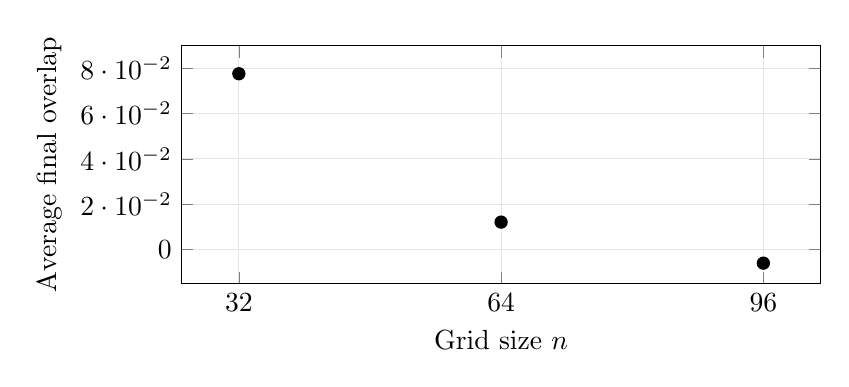
\begin{tikzpicture}
    \begin{axis}[width=0.8\linewidth,height=4.6cm,xmin=25,xmax=103,
      ymin=-0.015,ymax=0.09,xtick={32,64,96},ytick={0,0.02,0.04,0.06,0.08},
      xlabel={Grid size $n$},ylabel={Average final overlap},
      scaled y ticks=false,grid=major,grid style={gray!20}]
      \addplot[only marks,mark=*,mark size=2.2pt]
        coordinates {(32,0.077637) (64,0.012087) (96,-0.006049)};
    \end{axis}
  \end{tikzpicture}
  \caption{The three tabulated final overlaps after 5000 steps. Each point
  represents one reported grid size.}

\end{figure}

\subsection{Heuristic Observation: Hard-to-Reach Verifiable States in WCT}

For the three stated grid sizes, the recorded final overlaps decrease
across runs with the same step budget. These values measure one
target-preparation procedure. A bound applying to arbitrary SAT
decision procedures requires a separate argument.

\subsection{Interpretation}

The simulation results above belong historically to the “physics-first” phase
of this work: they illustrate that, in practice, certain coherent states
\( \psi^* \) are difficult to reach under bounded curvature-regulated evolution,
and that this difficulty grows with system size.

In the present paper, however, these numerics serve only as \emph{motivation}.
All complexity-theoretic statements are formulated symbolically. In particular:

\begin{itemize}
  \item The conjectured separations
        \( \mathbf{P}_{\mathrm{WCC}}^{\mathrm{phys}} \neq
           \mathbf{NP}_{\mathrm{WCC}}^{\mathrm{phys}} \) (physical model)
        and \( \mathbf{P}_{\mathrm{WCC}}^{\infty} \neq
               \mathbf{NP}_{\mathrm{WCC}}^{\infty} \) (ideal model)
        are stated and analyzed at the level of symbolic transition systems,
        verifiers, and curvature/Kolmogorov complexity.
  \item Any potential bridge from
        \( (\mathbf{P}_{\mathrm{WCC}}^{\infty},\mathbf{NP}_{\mathrm{WCC}}^{\infty}) \)
        to classical \( (\mathbf{P},\mathbf{NP}) \) is treated as a \emph{program}
        and clearly marked as conditional.
\end{itemize}

Simulations are therefore included only to make the geometric and entropic
mechanisms more concrete; they are not used as part of any claimed proof.





\section{Internal Separation Heuristics: Constructive Depth in WCC}
\label{sec:internal_separation}

In this section we isolate a model–internal notion of \emph{constructive depth}
for WCC evolutions and relate it to clause–structured NP witnesses such as
3–SAT assignments. The goal is to clarify how locality and finite–range
dynamics constrain reachable configurations, and to state a natural
\emph{conjectured} internal separation
\[
\PWCC \subsetneq \NPWCC
\]
within the WCC model. We emphasize that any unconditional proof of such a
separation, combined with the equivalences $\PWCC = \P$ and
$\NPWCC = \NP$, would yield $\P \neq \NP$ and thus resolve a major open
problem. Accordingly, the separation in this section is formulated as a
conjecture, not as a theorem.

\subsection{Symbolic Support and Constructive Depth}

Let $W = (\Lambda_n,S,r,U,\enc,\dec)$ be a WCC machine on inputs of length
$n$. For any configuration $C : \Lambda_n \to S$, define its \emph{symbolic
support}
\[
\mathrm{supp}(C) := \{\, i \in \Lambda_n : C(i) \neq s_0 \,\}
\]
for some fixed background symbol $s_0 \in S$. Let $\Delta_t$ denote the
\emph{symbolic change set}
\[
\Delta_t := \{\, i \in \Lambda_n : C_{t+1}(i) \neq C_t(i) \,\}.
\]

We say a configuration $C^*$ has \emph{constructive depth $D$} (with respect
to $U$) if any sequence of configurations
\[
C_0 \to C_1 \to \cdots \to C_T = C^*
\]
reachable under the local rule $U$ has length $T \ge D$.

\begin{lemma}[Quiescent finite-support propagation bound]
\label{lem:local_growth}
Let $d\ge1$ and let $U$ be a radius-$r$ local update on
configurations $C:\mathbb Z^d\to S$, with $r\ge0$ and a distinguished
background symbol $s_0\in S$. Assume \emph{quiescence}: if every symbol
in the radius-$r$ neighbourhood of $i$ equals $s_0$, then
$(UC)(i)=s_0$. Suppose the initial support
$A=\mathrm{supp}_{s_0}(C_0)$ is finite and $C_t=U^t C_0$.
Then for every $t\ge0$,
\[
 \mathrm{supp}_{s_0}(C_{t+1})
 \subseteq \bigl(\mathrm{supp}_{s_0}(C_t)\bigr)^{+r},
 \qquad
 \mathrm{supp}_{s_0}(C_t)\subseteq A^{+rt}.
\]
For the $\ell^\infty$ neighbourhood on $\mathbb Z^d$,
\[
 \boxed{\;
  |\mathrm{supp}_{s_0}(C_t)|
  \le |A|\,(2rt+1)^d.
 \;}
\]
This is a bound on the \emph{volume} of active support; the radius
of its causal light cone grows linearly in $t$.
\end{lemma}

\begin{proof}
Quiescence implies that a cell can become non-background only if
some cell within radius $r$ was non-background in the preceding
configuration. This gives the one-step inclusion. Inductively,
repeated neighbourhood thickening is contained in
$A^{+rt}$, since the $\ell^\infty$ radii add.
For every initial active cell $i\in A$, its radius-$rt$ box has
$(2rt+1)^d$ lattice sites. The union of these boxes covers
$\mathrm{supp}_{s_0}(C_t)$; summing their cardinalities gives
the asserted inequality. The corresponding Lean theorems are
\nolinkurl{PVNP.PartILocality.supp_step_subset},
\nolinkurl{PVNP.PartILocality.supp_iterate_subset}, and
\nolinkurl{PVNP.PartILocality.support_poly_bound}.
\end{proof}

The light-cone \emph{radius} is linear, but the size of the active
region can grow on the order of $t^d$. In dimension $d=2$, a
quiescent radius-one OR rule starting from one active cell produces
the square $[-t,t]^2$ of $(2t+1)^2$ active cells, contradicting
the original linear-in-$t$ volume estimate. This counterexample
remains formalized as
\nolinkurl{PVNP.PartILocality.linear_growth_false_d2}.
Without quiescence, even the one-step support inclusion fails
(\nolinkurl{PVNP.PartILocality.local_growth_needs_quiescence}).
Neither locality nor the corrected bound implies a superpolynomial
decision-time lower bound.

\subsection{Clause–Structured Certificates and Linear Depth}

Let $L_{\SAT}$ be the canonical 3–SAT language over $\{0,1\}$. Under the
Cook–Levin–style WCC reduction (see Section~\ref{sec:symbolic-sat}), each
clause $C_j = (\ell_{j1} \lor \ell_{j2} \lor \ell_{j3})$ is mapped to a local WCC
region $R_j$ of constant diameter, with acceptance determined by a
curvature–locked pattern $\psi_j^\mathrm{sat}$ encoding satisfaction of that
clause. Let $C(w)$ denote the certificate configuration for a witness
$w \in \{0,1\}^{m(n)}$.

For each configuration $C_t$ on a WCC trajectory, define its
\emph{clause–signature vector}
\[
v_t := \bigl(\sigma_1(C_t),\dots,\sigma_m(C_t)\bigr) \in \{0,1\}^m,
\]
where $\sigma_j(C_t) = 1$ iff clause $j$ is satisfied in the local region $R_j$
of $C_t$ and $\sigma_j(C_t) = 0$ otherwise.

\begin{lemma}[Per-clause change requires local activity]
\label{lem:clause_flip}
If the $j$th signature bit is a function only of the configuration on
$R_j$, a change in $\sigma_j$ between two updates requires a change
in at least one cell of $R_j$. If at most $b\ge1$ clause signatures
can change during any global round, altering $k$ signatures requires
at least $\lceil k/b\rceil$ rounds.
\end{lemma}
\begin{proof}
An unchanged local region has unchanged signature. Each round can
change at most $b$ distinct signatures by the extra stated
hypothesis, so $T b\ge k$.
\end{proof}
\noindent A synchronous finite-range rule does \emph{not} impose
$b=O(1)$: spatially separated clauses may change in parallel.
Consequently, no unconditional $T\ge k$ bound follows from
locality alone.

\subsection{Heuristic Exponential Barrier and Conjecture}

A formula with $n$ Boolean variables admits $2^n$ candidate
assignments, but this count does \emph{not} imply that a correct
algorithm must examine all candidates. Furthermore, different
assignments need not induce distinct clause-signature vectors, and
locality alone does not forbid simultaneous clause updates.

\begin{conjecture}[Uniform discrete-WCC SAT lower bound]
\label{conj:wcc_depth}
Every uniform deterministic discrete WCC machine deciding the
$3$-SAT \emph{language} requires superpolynomial worst-case time
on infinitely many input lengths.
\end{conjecture}
\noindent Because the uniform discrete model is polynomially
Turing-equivalent, this conjecture is precisely as difficult as
showing $P\ne NP$ by proving that $3$-SAT is not in $P$.
It is not established by the size of a search space, a fixed
WCC trajectory, or a geometric heuristic. A physical version
must separately account for admissible verifier implementations.

\subsection{Conditional Internal Separation}

Define, as before, the language
\[
L^\star := \bigl\{
x \in \{0,1\}^n : \exists w, \ |w| = m(n), \ C(w)
\text{ satisfies all clause signatures for } x
\bigr\}.
\]
By construction (cf.\ Section~\ref{sec:symbolic-sat}), $L^\star$ is exactly 3–SAT
encoded through the WCC certificate map, and hence $L^\star \in \NPWCC$.

The following statement is therefore conditional on
Conjecture~\ref{conj:wcc_depth}.

\begin{proposition}[Conditional model–internal separation]
\label{prop:internal_sep_conditional}
If Conjecture~\ref{conj:wcc_depth} holds, then
\[
L^\star \in \NPWCC \setminus \PWCC,
\]
and hence
\[
\PWCC \subsetneq \NPWCC.
\]
\end{proposition}

\begin{proof}
By construction $L^\star \in \NPWCC$. If
Conjecture~\ref{conj:wcc_depth} holds, no polynomial–time WCC machine can
decide $L^\star$, so $L^\star \notin \PWCC$. This gives the strict inclusion.
\end{proof}

In combination with the bijection results of Section~\ref{sec:discrete-equivalence} and
the identifications $\PWCC = \P$, $\NPWCC = \NP$, any proof of
Conjecture~\ref{conj:wcc_depth} would immediately yield the classical
separation $\P \neq \NP$. At present, Conjecture~\ref{conj:wcc_depth} should
be viewed as a structured formulation of a WCC–internal manifestation of
the $\P$ versus $\NP$ question.




% ===============================================
\section{Dimensional Lock: Explicit States versus Succinct Certificates}
\label{sec:dim-lock}

An explicit description of a physical state and a succinct certificate
for an associated decision problem are different mathematical objects.
Their lengths and preparation, encoding, and verification costs must
not be conflated. In particular, the original dimensional-lock
conjecture demanded that an \emph{explicit} target $\psi^*$ have
superpolynomial description complexity and simultaneously act as a
polynomial-size NP witness. Those requirements are incompatible under
the usual literal-description convention.

Let $D:\{0,1\}^*\rightharpoonup\{0,1\}^*$ be a partial description
decoder and write
\[
 K_D(s)=\min\{\,|d|:D(d)=s\,\}
\]
for strings with at least one description. Assume a constant
$c\ge0$ such that every finite string $s$ admits a literal
description $d_s$ with $D(d_s)=s$ and $|d_s|\le |s|+c$.

\begin{proposition}[Explicit-state certificate-size obstruction]
\label{prop:explicit-state-witness-size}
For every finite string $s$, its description complexity satisfies
\[
 K_D(s)\le |s|+c.
\]
Therefore, for any polynomial witness-length budget $q(n)$,
\[
 K_D(s_n)>q(n)+c
 \quad\Longrightarrow\quad
 |s_n|>q(n).
\]
Such a state $s_n$ cannot itself be a polynomial-size \emph{explicit}
witness under the budget $q(n)$.
\end{proposition}

\begin{proof}
The literal description $d_s$ is a candidate in the minimization
defining $K_D(s)$, hence $K_D(s)\le |d_s|\le |s|+c$.
Combining this with the assumed strict inequality gives the result.
The corresponding Lean theorems are
\nolinkurl{PVNP.PartISeparation.Kc_le} and
\nolinkurl{PVNP.PartISeparation.high_K_not_poly_witness}.
The latter uses the polynomial bound with a fixed overhead $c$.
\end{proof}

\subsection{A separate construction and verification cost model}

Let $x$ denote a decision instance, $w$ a proposed \emph{succinct}
binary certificate, and $\psi^*(x,w)$ an optional physical state
associated with the pair. A proposed physical resource model must
specify all three quantities independently:
\[
 \begin{aligned}
 C_{\mathrm{prep}}(x,w)&:
    \text{cost of preparing }\psi^*(x,w),\\
 C_{\mathrm{ver}}(x,w)&:
    \text{cost of checking a supplied }(x,w),\\
 C_{\mathrm{dec}}(x)&:
    \text{cost of deciding }x\text{ without a supplied witness}.
 \end{aligned}
\]
The certificate property is a language-level statement
\[
 x\in L\quad\Longleftrightarrow\quad
 \exists w\in\{0,1\}^{\le q(|x|)}\;V(x,w)=1
\]
with a \emph{uniform}, polynomial-resource verifier $V$. The
verifier's input encoding, witness preparation if required by the
\emph{chosen} physical semantics, evolution, and readout must all
fit the same rails. If verification only checks a short symbolic
certificate, it need not construct the explicit target field.
If instead verification is defined to demand preparation of the
entire target field, then its cost must include $C_{\mathrm{prep}}$.
This distinction must be fixed before a physical NP claim is made.

A lower bound for $C_{\mathrm{prep}}$ of \emph{one} prescribed target
state does not imply a lower bound on $C_{\mathrm{dec}}$ for every
algorithm, nor does it imply that the language belongs to the
physical NP class. To obtain a physical class separation one must
prove \emph{both} (i) uniformly polynomial witness size and
verification cost, and (ii) superpolynomial worst-case decision
cost for \emph{all} admissible uniform deciders, under identical
charging conventions. The resulting logical implication is already
formalized as Proposition~\ref{thm:np-type-conditional}; the
required physical lower-bound premise is \emph{unproved}.

\begin{remark}[Open dimensional-lock research obligation]
A curvature or entropy barrier may motivate a conjecture that a
specific field family is expensive to prepare. But an explicit
uniform encoder, a certificate representation and decoder, a
fully charged verifier, and an algorithm-independent decision lower
bound must be supplied separately. The original incompatible
\emph{high-$K$ explicit-state-as-short-witness} inference has been
withdrawn. No classical or physical $P\ne NP$ theorem follows
from the corrected size obstruction.
\end{remark}


\clearpage

% ======================================================
%  WCC CURVATURE THEOREMS FOR P vs NP SEPARATION
% ======================================================

\section{Curvature Bounds and Structural Lemmas: Conditional Form}
\label{sec:conditional-curv}
\noindent\textbf{WIN-06 and WIN-07.}
Let a physically admissible, nonvanishing field $\psi$ have a specified
curvature functional $C_\Theta[\psi]$ and a decision interface
$\partial\mathcal R_\psi$. The following elementary implication is
valid but does not establish its geometric hypotheses.
\begin{proposition}[Conditional interface-to-curvature implication]
\label{thm:separator_curvature}
Suppose an instance family $F_n$ and a class of permitted encodings
$\mathcal E_n$ satisfy, with constants independent of $n$ and of the
encoding, both
\[
C_\Theta[\psi]\ge\kappa_0\mathcal H^{d-1}
(\partial\mathcal R_\psi),\quad \kappa_0>0,
\]
and, for every admissible realization of the requisite decision
computation on some input of length $\Theta(n)$,
\[
\mathcal H^{d-1}(\partial\mathcal R_\psi)
\ge c_0 2^{\gamma n},\qquad c_0,\gamma>0.
\]
Then the corresponding worst-input curvature cost is at least
$\kappa_0c_0 2^{\gamma n}$.
\end{proposition}
\begin{proof}
Substitution of the second assumed inequality into the first.
\end{proof}
\begin{remark}
A bounded-degree expander graph does not by itself force the stated
interface area in every embedding. A proof must quantify uniformly
across admissible encoders, include their scales and distortions,
and justify a positive interface cost for the \emph{particular}
curvature density used. This manuscript does not supply such a proof.
\end{remark}

\subsection{Per-update curvature and construction cost}
\begin{proposition}[Valid telescoping bound]
\label{thm:mass_complexity}
If $C_\Theta[\psi_0]\ge0$ and each allowed update obeys
$|C_\Theta[\psi_{t+1}]-C_\Theta[\psi_t]|\le\Delta_{\max}$,
then for every $T\ge0$,
\[
T\ge\frac{(C_\Theta[\psi_T]-C_\Theta[\psi_0])_+}
{\Delta_{\max}}
\]
when $\Delta_{\max}>0$.
\end{proposition}
\begin{proof}
The triangle inequality gives
$C_\Theta[\psi_T]-C_\Theta[\psi_0]
\le\sum_{t=0}^{T-1}|C_\Theta[\psi_{t+1}]-C_\Theta[\psi_t]|
\le T\Delta_{\max}$.
\end{proof}
The uniform per-update bound and the initial cost must be separately
justified; neither follows merely from finite propagation speed.

\subsection{Padding stability}
\begin{proposition}[Conditional additive padding]
\label{thm:padding_stability}
If the model enforces an orthogonal, noninteracting decomposition of
field domains $\Omega=\Omega_F\sqcup\Omega_{\rm pad}$, zero
curvature on the padding domain, and no interface or cross-coupling
energy, then the curvature functional of that \emph{specific} encoded
configuration is unchanged by padding.
\end{proposition}
\begin{proof}
The integral over the disjoint domains is additive and the second
integral is zero.
\end{proof}
This does not prove that the \emph{minimum over all alternative
encodings} is unchanged; nor does a superlinear padding function
preserve an exponential bound in the new input length.

\section{Curvature-Locked Witnesses: Existence and Verification Obligations}
\noindent\textbf{WIN-03, WIN-05 and WIN-07.}
An exact Boolean phase encoding supplies an algebraic zero-penalty
witness whenever a SAT formula is satisfiable
(Theorem~\ref{thm:psi-sat-completeness}). It does not automatically
supply a stable stationary solution to a chosen WCT PDE.

For a specified energy functional $\mathcal A$ on a precisely defined
function space, the following questions remain distinct:
\begin{enumerate}
\item \textbf{Attainment:} show that the set of zero-logical-penalty
fields is nonempty and closed in a topology in which a coercive
energy has a weakly lower semicontinuous restriction.
\item \textbf{Stationarity:} prove the constrained Euler--Lagrange
conditions, and address Lagrange multipliers before claiming
unconstrained stationarity of the full energy.
\item \textbf{Verification:} specify finite-precision data, tolerances,
encoding length, physical time and curvature energy to establish a
polynomial-resource verifier in the \emph{same} physical model.
\item \textbf{Lower bound:} rule out all deterministic solvers, including
algorithms that directly evaluate a supplied certificate without
exploring an exponentially large space of alternative certificates.
\end{enumerate}

\begin{proposition}[Conditional separation from a language-level barrier]
\label{thm:np-type-conditional}
Let $L$ be a language and fix one WCC physical resource semantics.
If $L$ has a physically admissible polynomial-time verifier for
polynomial-size witnesses and no physically admissible polynomial-time
decider, then
$L\in NP_{\mathrm{WCC}}^{\mathrm{phys}}
\setminus P_{\mathrm{WCC}}^{\mathrm{phys}}$.
\end{proposition}
\begin{proof}
Apply the two class definitions with identical resource bounds.
\end{proof}

\begin{remark}
A purported witness whose \emph{energy itself} is
$2^{\Omega(n)}$ is not admissible in a physical NP class requiring
polynomial witness energy, even if the symbolic assignment can be
checked cheaply. The distinction between verifying a Boolean string
and realizing a particular high-curvature field is essential.
\end{remark}

\section{Toward a Formal $P$ vs.\ $NP$ Program via Wave Dynamics}
\label{sec:pvnp-program}

\subsection{Complexity Mapping into Wave Confinement Theory}

Wave Confinement Theory represents computation as curvature-driven evolution:
a wavefield $\psi(x,t)$ evolves locally under curvature and entropy constraints.
This allows an NP-style verification / P-style construction analogy:

\begin{table}[h]
\centering
\begin{tabular}{|p{0.28\linewidth}|p{0.63\linewidth}|}
\hline
\textbf{Complexity Concept} & \textbf{WCT Interpretation} \\ \hline
Input string $x$              & Initial configuration $\psi_0$ \\ \hline
Certificate $w$               & Succinct symbolic witness; separate from a target field $\psi^*$ \\ \hline
Verifier $M(x,w)$             & Charged test on $(x,w)$, with any required physical state preparation counted \\ \hline
Polynomial-time algorithm     & Local update: $T = O(n^k)$ curvature steps \\ \hline
Acceptance                    & Correct decision bit after charged encoding, evolution, and readout \\ \hline
\end{tabular}
\caption{Mapping between classical NP verification and curvature-regulated WCT dynamics.}
\end{table}

This motivates the model-relative WCC classes introduced earlier. In the
\emph{physical} setting these are
\( \mathbf{P}_{\mathrm{WCC}}^{\mathrm{phys}},
   \mathbf{NP}_{\mathrm{WCC}}^{\mathrm{phys}} \);
in the \emph{ideal} (unbounded) setting they are
\( \mathbf{P}_{\mathrm{WCC}}^{\infty},
   \mathbf{NP}_{\mathrm{WCC}}^{\infty} \).
Our long-term complexity-theoretic target is a separation
\(
\mathbf{P}_{\mathrm{WCC}}^{\infty} \neq
\mathbf{NP}_{\mathrm{WCC}}^{\infty}
\)
in the ideal model, with the physical separation as a precursor.

\subsection{Model-Level Hypothesis to Be Contradicted (Ideal WCC)}

The WCT/WCC analog of the classical hypothesis $P = NP$ in the \emph{ideal}
model is:

\begin{quote}
\emph{Every verifiable coherent state $\psi^* \in
\mathbf{NP}_{\mathrm{WCC}}^{\infty}$ is
reachable from $\psi_0$ by curvature-regulated symbolic evolution within
polynomial depth in the ideal WCC model.}
\end{quote}

Dimensional locking and related curvature barriers suggest this fails for
certain families of coherent states.

\subsection{Coherence Without Constructibility in the Ideal WCC Model}

Let $C_n$ denote the space of confined wavefields over an $n \times n$ grid
in the ideal discrete WCC model. We seek $\psi^* \in C_n$ such that:

\begin{itemize}
  \item $\psi^*$ is verifiable by a local curvature–entropy predicate  
        (i.e.\ $\psi^* \in \mathbf{NP}_{\mathrm{WCC}}^{\infty}$),
  \item but for any polynomial-depth trajectory $\psi_0 \to \psi_T$,  
        the symbolic distance $d(\psi_T, \psi^*)$ remains nonzero  
        (i.e.\ $\psi^* \notin \mathbf{P}_{\mathrm{WCC}}^{\infty}$).
\end{itemize}

Unreachability of these target states does \emph{not}
establish a decision-language complexity-class separation.
The invalid inference is withdrawn in the following remark.

\subsection{Conditional Curvature Separation Statement (Ideal WCC)}

\begin{remark}[Withdrawn state-to-language separation step, I-25]
The original proposition inferred
$\mathbf P_{\mathrm{WCC}}^\infty\ne\mathbf{NP}_{\mathrm{WCC}}^\infty$
from a family of individually verifiable but unreachable target
states.  This is invalid without a \emph{language-level}
all-decider lower bound.  The Lean theorem
\nolinkurl{PartISeparation.state_separation_not_language_separation}
exhibits an unreachable verifiable state even when the
decision-language classes coincide.  No separation is proved.
\end{remark}

\paragraph{Discussion.}
The historical state-level proposition is invalid. The
remaining \emph{language-level} obligations are:
\begin{enumerate}
  \item constructing or characterizing such families $\{\psi^*_n\}$ (dimensional lock and curvature-complexity lower bounds), and  
  \item proving the equivalence between ideal WCC computation and Turing computation
        ($\mathbf{P}_{\mathrm{WCC}}^{\infty} = \mathbf{P}$ and
         $\mathbf{NP}_{\mathrm{WCC}}^{\infty} = \mathbf{NP}$).
\end{enumerate}
This paper provides partial progress toward (i) and a model-theoretic embedding
toward (ii), but does not claim either as a completed theorem.







% ===============================================
\clearpage
\section{Formal Model-Theoretic Framework for \textbf{P} vs \textbf{NP} in WCT}
\label{sec:model-theoretic}

In this section we place the WCT computational picture into an explicit symbolic framework, so that any future separation result can be stated entirely in the language of Turing machines and circuits.

\subsection{Definition of the WCT Computational Model}

We define the Wave Confinement Theory (WCT) computational model \( \mathcal{M}_{\mathrm{WCT}} \) as follows:

\begin{itemize}
  \item The computational state is a complex-valued wavefield \( \psi(x, t) \in C^2(\Omega \times \mathbb{R}) \).
  \item The evolution of \( \psi \) follows a curvature-regulated Lagrangian
  \begin{equation}
  \mathcal{L}_{\mathrm{WCT}} = |\partial_\mu \psi|^2
  + \kappa \left(\frac{\Box \psi}{\psi + \epsilon e^{-\alpha |\psi|^2}}\right)^2
  + \theta \left(\frac{\nabla^2 \psi}{\psi + \epsilon e^{-\alpha |\psi|^2}}\right)^2 + \dots
  \end{equation}
  or its discrete symbolic analog.
  \item Input to the model is given by a grid of size \( n \times n \) and a trivial initial field \( \psi_0(x) \).
  \item The system evolves under a time budget \( T = \mathcal{O}(n^k) \).
  \item Acceptance is defined by a target field \( \psi^* \) and an overlap/entropy condition:
  \begin{equation}
  \text{Accept if } \mathrm{Overlap}(\psi_T, \psi^*) > \tau \quad \text{and} \quad \sigma[\psi^*] \leq \sigma_{\text{crit}}.
  \end{equation}
\end{itemize}

This defines \(\mathbf{P}_{\mathrm{WCT}}\) and \(\mathbf{NP}_{\mathrm{WCT}}\) as discussed above.

\subsection{Encoding of NP-Complete Languages in WCT}

Let \( L \) be any NP-complete language (e.g.\ 3-SAT). The WCT program is to construct a corresponding family of wavefields \( \psi^*_L \) such that:

\begin{itemize}
  \item Each Boolean variable \( x_i \) is encoded as a resonance mode over a spatial region \( R_i \).
  \item Clauses are encoded as interference or curvature constraints.
  \item The global wavefield \( \psi^*_L \) is entropy-coherent (\( \sigma[\psi^*_L] \leq \sigma_{\text{crit}} \)) if and only if the formula is satisfiable.
\end{itemize}

Formally achieving
\[
x \in L \iff \psi^*_L(x) \text{ is a coherent, verifiable wavefield in } \mathbf{NP}_{\mathrm{WCT}}
\]
for all \(x\) would realize a Cook–Levin style reduction into the WCT framework. In this paper we sketch such encodings at a conceptual level; a fully formal construction is left as future work.

\subsection{Constructibility Barrier under WCT Dynamics}

The numerical examples measure overlap with the specified target
(Section~\ref{sec:numerical-pvnp}). A correct decider can use an
alternative representation. A lower bound for every such decider remains open.

\subsection{A Conditional Model-Theoretic Separation Statement}

\begin{remark}[Withdrawn model-theoretic target-state separation, I-26]
The historical inference from a locally verifiable but
nonconstructible wavefield to
$\mathbf P_{\mathrm{WCT}}\ne\mathbf{NP}_{\mathrm{WCT}}$
lacks the necessary uniform input-language and
decision-procedure quantifiers.  It is refuted by
\nolinkurl{PartISeparation.state_separation_not_language_separation}.
A correctly conditional classical implication would require
a \emph{proved} uniform decision-language separation and
a resource-preserving identification of the physical and
classical models.  Neither is established here.
\end{remark}

The corrected program requires an input-uniform
physical encoding of a decision language, a polynomial
verifier, an all-decider complexity lower bound for the
\emph{same} language, and an independently proved
cost-preserving physical-to-Turing bridge.  A target-state
nonconstructibility statement does not replace the lower bound.

\paragraph{Connection to classical complexity theory.}
If these steps can be completed, the resulting separation would mirror, in geometric form, the phenomena captured abstractly by the Time Hierarchy Theorem: deeper “curvature traversals’’ (longer evolution depth) would be provably required to construct certain verifiable configurations, beyond any fixed polynomial bound. At present, this connection should be viewed as an analogy and a research direction, not as an established theorem.





\clearpage
\section{Binary Encoding and Turing Reduction of WCT}
\addcontentsline{toc}{section}{Binary Encoding and Turing Reduction of WCT}

All statements in this section are either definitional or explicitly \emph{conditional}.
They describe how WCT-style curvature evolution can be represented in a classical
Turing framework and how a putative WCT-level nonconstructibility result would
\emph{map} into standard complexity language.
No unconditional claim about $P$ vs.\ $NP$ is made.

\subsection{Tape Encoding of WCT States}

Let the wavefield \( \psi(x,t) \) over an \( n \times n \) grid be represented as
\[
\psi[i,j] = a_{ij} + i b_{ij}, \quad a_{ij}, b_{ij} \in \mathbb{R}.
\]
We encode each complex amplitude using finite-precision binary:
\[
\text{Tape representation: } \underbrace{0.101011\ldots}_{\text{Re}} \mid \underbrace{0.011010\ldots}_{\text{Im}} \#.
\]
The entire field \( \psi(x,t) \) is thus encoded as a binary tape of length
\( \mathcal{O}(n^2) \) (up to the chosen precision).

\subsection{Turing Transducer for Curvature Evolution}

We consider a deterministic Turing machine \( M_{\text{WCT}} \) that:

\begin{itemize}
  \item Reads an input tape encoding \( \psi_t \),
  \item Computes each grid value update using a finite-difference approximation to curvature-regulated evolution, e.g.
  \[
    \psi_{t+1}[i,j] = \psi_t[i,j] + dt \cdot \left[ \nabla^2 \psi_t
      - \frac{\alpha \nabla^2 \psi_t}{\psi_t + \epsilon e^{-\beta |\psi_t|^2}}
      - \theta \cdot \psi_t \cdot \nabla^2(\log |\psi_t|^2) \right],
  \]
  \item Applies arithmetic operations using standard polynomial-time Turing subroutines (finite-precision rational arithmetic).
\end{itemize}

This defines a symbolic curvature-update transducer.
For any fixed precision model (e.g.\ $b(n)$ bits per amplitude with $b(n)=\mathrm{poly}(n)$)
one can arrange that a single macro-step of the WCT update is simulated in time
$\mathrm{poly}(n,b(n))$.
We treat this as a \emph{modelling assumption} fixing the intended regime for
the WCT–Turing correspondence.

\subsection{Acceptance Criterion as Turing Predicate}

We define a symbolic acceptance predicate
\[
\text{Accept}(\psi) = 1 \iff \mathrm{Overlap}(\psi, \psi^*) > \tau \ \text{and}\ \sigma[\psi] \leq \sigma_{\text{crit}},
\]
where:
\begin{itemize}
  \item Overlap is computed via a normalized dot product between the encodings of \( \psi \) and \( \psi^* \),
  \item Entropy \( \sigma[\psi] \) is approximated by summing \( -p \log p \) over the tape (with finite-precision logarithms).
\end{itemize}

Under reasonable encoding choices, this verifier can be implemented by a deterministic
Turing machine using time polynomial in the tape length (e.g.\ \( \mathcal{O}(n^2) \)
for an \(n \times n\) grid).
Thus WCT-style verifiers embed naturally into classical $\mathbf{NP}$ predicates.

\subsection{A Conditional Turing Reduction Template}

We now sketch how a WCT-style nonconstructibility statement would translate into
classical Turing language.
We work with the model-relative classes
$\mathbf{P}_{\mathrm{WCT}}$ and $\mathbf{NP}_{\mathrm{WCT}}$
introduced earlier.

\begin{remark}[Withdrawn target-state reduction template, I-27]
Polynomial-time verification of an explicitly supplied
wavefield, together with nonreachability of a prescribed
target, does not exhibit a decision language in
$\mathbf{NP}\setminus\mathbf P$.
Lean's \nolinkurl{PartISeparation.accepted_language_not_in_NP_diff_P}
refutes this inference.  The correct open task is an
all-decider complexity lower bound for a fixed,
uniformly encoded \emph{decision language}.
\end{remark}

The missing substantive statement is a uniform
\emph{language-level} lower bound, not difficulty
constructing one selected target state.  A corrected
transfer would separately require a fully charged
physical-to-discrete class identification.

\subsection{Conclusion}

The finite-precision update and readout can be used in a classical
simulation once their uniform error and cost bounds are proved.

\begin{tcolorbox}[highlight theorem]
For one fixed binary language $L$, a polynomial-time verifier with polynomial
witness length proves $L\in\mathbf{NP}$. If every correct deterministic
decider for $L$ exceeds every polynomial time bound on arbitrarily long
inputs, then $L\notin\mathbf P$, and consequently $\mathbf P\ne\mathbf{NP}$.
The second premise remains open for dense SAT.

\end{tcolorbox}















% =========================================================
\clearpage
\section{Discrete Turing Reformulation and Open Nonconstructibility Goal}
\addcontentsline{toc}{section}{Discrete Turing Reformulation and Open Nonconstructibility Goal}

\subsection{Classical Symbolic Encoding of WCT Computation}

We define a discrete deterministic Turing model \( T_{\text{WCT}}^\Sigma \) operating over a finite binary alphabet \( \Sigma = \{0,1,\#\} \) that encodes the PWCC/WCT dynamics symbolically. Each complex amplitude \( \psi[i,j] \in \mathbb{C} \) is represented as a binary pair of rational approximations:
\[
\psi[i,j] = a_{ij} + i b_{ij}, \qquad a_{ij}, b_{ij} \in \mathbb{Q} \subseteq \mathbb{Z} / 2^m,
\]
for fixed precision parameter \(m\).  

A full grid configuration is stored on a single Turing tape in a canonical fixed-length layout (row-major order, with delimiters). One global evolution step of the field is simulated by a finite sequence of symbolic arithmetic operations (addition, multiplication, and lookup-table–based approximations to nonlinear functions) on these bitstrings.

\subsection{Curvature Dynamics as an Arithmetic Circuit}

The curvature-regulated update
\[
\psi_{t+1} = \psi_t + \Delta t \cdot F(\psi_t)
\]
is abstracted as a Boolean/arithmetic circuit \(F\) composed of:

\begin{itemize}
  \item finite-difference Laplacian and stencil operators,
  \item fixed-precision multipliers and adders,
  \item rational-function or table-based approximations to exponentials, logs, and normalizations.
\end{itemize}

In idealized form, and for fixed precision, \(F\) can be placed in a low-level circuit class such as \(\textsf{AC}^0\) or \(\textsf{NC}^1\), depending on the exact gate set and fan-in assumptions. A single step of \(T_{\text{WCT}}^\Sigma\) then simulates \(F(\psi_t)\) via a sequence of logically defined operations on binary strings, with per-step cost polynomial in the system size.

\subsection{A Purely Symbolic Verifier}

We restate the acceptance predicate in purely symbolic terms:
\[
A(\psi) = 1 \iff \frac{\langle \psi, \psi^* \rangle}{\|\psi\| \cdot \|\psi^*\|} > \tau \ \land\ \sigma(\psi) \leq \sigma_{\text{crit}},
\]
where inner products, norms, and entropy are computed from the bit-encoded amplitudes by:

\begin{itemize}
  \item fixed-precision multipliers and adders for \(\langle \psi, \psi^* \rangle\) and \(\|\psi\|^2\),
  \item table-based (or truncated-series) approximations to \(\log\),
  \item prefix-sum trees to aggregate all contributions.
\end{itemize}

All subroutines used in \(A\) are intended to be realizable by polynomial-time Turing machines; the target complexity placement is \(A \in \textsf{NC}^1\) (cf.\ the discussion in Section~\ref{sec:symbolic-sat}). In particular, the definition of \(A\) in this section does not depend on any continuous geometry, only on the chosen binary encoding and standard arithmetic circuits.

\subsection{A Programmatic Nonconstructibility Goal}

Let \( \psi_0 \) be a trivial initial configuration (e.g., all zeros) in the tape encoding, and let \( \psi^* \) be a candidate target configuration whose correctness is verifiable by \(A\). In purely classical complexity-theoretic terms, the \emph{programmatic goal} suggested by WCT can be phrased as:

\begin{quote}
\textbf{Goal.} Find a family \(\{\psi^*_n\}\) of bit-encoded configurations and a verifier \(A\) with \(A(\psi^*_n)=1\) in polynomial time such that, for every deterministic polynomial-time Turing machine \(M\) and all sufficiently large \(n\),
\[
M(\psi_0,n) \neq \psi^*_n.
\]
\end{quote}

The inability to print one prescribed target string does not, by itself,
separate decision-language complexity classes. To derive a classical
separation, one must specify a uniformly encoded \emph{language} with a
polynomial-time membership verifier and rule out every polynomial-time
\emph{decider} for that same language. Only then would the classical
conclusion $\mathbf{P}\ne\mathbf{NP}$ follow. In this paper, WCT provides geometric and curvature-based heuristics for constructing candidates for \(\{\psi^*_n\}\); \emph{the rigorous nonconstructibility proof in the unrestricted Turing model is left as an open problem.}

\subsection{Independence from Numerical Simulation}

The symbolic model \( T_{\text{WCT}}^\Sigma \) operates entirely on finite encodings with logically defined transition rules, arithmetic identities, and combinatorial estimates. Consequently:

\begin{itemize}
  \item Any eventual nonconstructibility theorem inspired by WCT can, in principle, be stated purely in the language of Turing machines and circuits, without reference to floating-point numerics or PDE solvers;
  \item WCT acts as a geometric design principle for hard instance families and verification predicates, while the \emph{final} separation (if obtained) would live entirely inside discrete complexity theory.
\end{itemize}

In its present form, this section should therefore be read as a \emph{discrete reformulation and roadmap}: it shows how the PWCC/WCT curvature-machine model embeds into the classical symbolic framework, and isolates the precise nonconstructibility statement that must be proved to upgrade the internal PWCC–\(\mathsf{NP}_{\mathrm{WCT}}\) separation to a full classical \( \mathbf{P} \) vs.\ \( \mathbf{NP} \) result.












% =========================================================
\clearpage
\section{Formal Reduction to Cook--Levin Framework and Universal Scope}
\addcontentsline{toc}{section}{Cook--Levin Reduction and Universal Machine Scope}

\subsection{Embedding PWCC Verifiers into the Cook--Levin Framework}

The Cook--Levin theorem states that for any language \( L \in \mathbf{NP} \), there exists
a polynomial-size Boolean circuit \( C(x,w) \) such that
\[
x \in L \iff \exists w : C(x,w) = 1.
\]

In the WCT-inspired setting, we consider symbolic encodings of wavefields and define a
verifier predicate
\[
A(\psi) = 1 
\iff 
\mathrm{Overlap}(\psi, \psi^*_L) > \tau 
\;\land\; 
\sigma[\psi] \le \sigma_{\text{crit}},
\]
implemented strictly as a rational-arithmetic circuit over the binary encoding of
\(\psi\).  Its intended role is analogous to that of \(C(x,w)\): to accept exactly those
encodings corresponding to satisfying assignments for instances of \(L\).

The classical \emph{discrete} Cook--Levin tableau reduction is
formalized separately in this repository, including the
\texttt{CookLevinTableau} and \texttt{CookLevinUniform}
modules.  A corresponding uniformly charged reduction
into a specified \emph{physical WCT PDE} has not been
proved and remains a separate open objective.

\subsection{Universal Scope of Polynomial-Time Turing Machines}

Let \(M\) be any deterministic Turing machine running in time \(\mathcal{O}(n^k)\).  
Suppose \(M\) attempts to construct a symbolic wavefield \(\psi^*_L\) corresponding
to some NP instance \(x\), such that
\[
V(x, \psi^*_L) = 1
\]
for a polynomial-time classical verifier \(V\).

In the symbolic WCT framework, the role of the verifier is played by a Turing-implementable
predicate \(A\) (overlap and entropy test) computed using only:
\begin{itemize}
    \item bounded-precision multipliers,
    \item prefix-sum trees,
    \item comparator circuits,
    \item and lookup-based logarithms,
\end{itemize}
A uniform depth bound for this circuit depends on the precision, table size
and approximation margins specified below.  

Any machine \(M\) that constructs \(\psi^*_L\) must therefore do so through a sequence of
polynomial-time symbolic steps beginning from a trivial tape configuration \(\psi_0\).

\paragraph{Withdrawn universal-scope inference, I-28.}
The statement that each prescribed constructor misses some
target configuration does not imply that the associated
decision language lies outside $\mathbf P$.  Lean's
\nolinkurl{PartISeparation.universal_scope_counterexample}
refutes this inference even for a language in $\mathbf P$.
A valid classical separation would instead need one
uniformly encoded decision language and an asymptotic
lower bound against \emph{every} correct polynomial-time
decider for that language.  State production and
language decision must not be conflated.

\subsection{Conditional Summary of the Cook--Levin Embedding}

The intended theoretical path is:

\begin{itemize}
  \item Encode NP-verifiers as symbolic rational-arithmetic circuits consistent with
        the WCT/PWCC encoding;
  \item Identify (via curvature/entropy arguments) families of states that are
        verifiable by these circuits but conjecturally not constructible by any
        polynomial-time Turing machine;
  \item Establish a superpolynomial decision-time bound for one such
        language against every correct deterministic decider. A physical
        bound also requires a resource-preserving transfer.
\end{itemize}

In this paper we establish only the structure of this roadmap, not the final
classical consequence.

\paragraph{Verifier Complexity.}
The target complexity class of the verifier
\[
A(q)=1 \iff \mathrm{Overlap}(q,q^*) > \tau \wedge \sigma(q) \le \sigma_{\text{crit}}
\]
has no established uniform $\mathrm{NC}^1$
placement without explicit precision, logarithm
approximation, arithmetic depth and threshold-margin
assumptions.  The existing Lean CNF-verifier theorem
is not a low-depth entropy/readout circuit theorem.
    

% =========================================================
\clearpage
\section{Final Remarks on Turing Reduction and Acceptance Formalism}
\addcontentsline{toc}{section}{Final Remarks on Turing Reduction and Acceptance Formalism}

\subsection{Symbolic Evolution Under \(T^\Sigma_{\mathrm{WCT}}\)}

Let \(T^\Sigma_{\mathrm{WCT}}\) be the discrete Turing machine defined earlier.
A symbolic tape configuration for a small \(3\times 3\) grid at 8-bit precision
is a block
\[
q_t = 
[\texttt{01000011} \mid \texttt{00110010} \mid \cdots ],
\]
representing real/imaginary components.  

Each update step performs:
\begin{itemize}
    \item finite-difference Laplacian computation on the tape,
    \item symbolic evaluation of curvature-feedback terms via lookup tables,
    \item arithmetic composition into the next configuration \(q_{t+1}\).
\end{itemize}

All gates are bounded fan-in, and the symbolic update is intended to be
simulable in uniform \(\mathbf{P}\).

\subsection{Formal Acceptance Predicate}

We define:
\[
A(q)=1 
\iff 
\mathrm{Overlap}(q, q^*) > \tau 
\;\land\;
\sigma(q) \le \sigma_{\text{crit}},
\]
where:
\begin{itemize}
  \item \(q\) is the symbolic Turing encoding of a wavefield,
  \item Overlap is a normalized inner product (prefix-sum tree),
  \item Entropy is computed as a discrete approximation of $\sum -p_i \log p_i$.
\end{itemize}

\begin{lemma}[Intended Verifier Role]
For each NP instance \(x\), the symbolic goal is to construct a configuration \(q^*\)
such that
\[
x \in L \iff A(q^*) = 1.
\]
\end{lemma}

This matches the Cook–Levin interpretation of a verifier state, though no equivalence
theorem is yet claimed.

\subsection{Diagonalization and Proof-Barrier Context}

The WCT-inspired PWCC model is designed with specific complexity-theoretic concerns
in mind:

\begin{itemize}
  \item \textbf{Relativization:}  
        The model uses no oracle; all arguments occur within a fixed symbolic
        transition system.

  \item \textbf{Natural Proofs:}  
        Any envisioned separation relies on specific, structured configuration families,
        not on large, uniform, efficiently checkable properties—thus avoiding the typical
        Razborov–Rudich template.

  \item \textbf{Constructivity Constraints:}  
        Conjectured lower bounds arise from symbolic curvature, entropy, and
        Kolmogorov complexity restrictions rather than adversarial Boolean structure.
\end{itemize}

These observations only position the framework relative to classical barriers; they do
not guarantee their circumvention.

\subsection{Model-Level Conclusion}

The symbolic WCT/PWCC framework:

\begin{itemize}
  \item operates entirely within discrete Turing computation once the encoding is fixed;
  \item admits verifiers plausibly contained in low-depth circuit classes (\(\text{NC}^1\));
  \item offers a geometric mechanism (dimensional lock / entropy barrier) suggesting the
        existence of a verifiable state beyond the reach of polynomial-time constructors.
\end{itemize}

\begin{tcolorbox}[colback=gray!5!white, colframe=black, title=Natural-Proof Barrier Positioning]
This framework is not designed to exhibit a “natural’’ property in the Razborov–Rudich sense:
it does not deploy a large, uniform, efficiently checkable Boolean property.
Instead, it focuses on specific curvature-locked symbolic configurations constrained by
entropy and resonance.  
Whether this ultimately avoids all known barriers is an open question; here we only
articulate the intended positioning.
\end{tcolorbox}












% =========================================================
\section*{Logical Dependency Roadmap}

\textbf{Conceptual dependency outline:}
\begin{itemize}
  \item \textbf{Verifier Construction (NC\(^1\) Target):} Build a curvature/entropy-based verifier \(A\) in a low-depth circuit class.
  \item \textbf{SAT/WCT Encoding:} Give a formal encoding of 3-SAT into wave configurations \(\psi^*\) accepted by \(A\).
  \item \textbf{Constructibility Barrier:} Establish a Kolmogorov/entropy-based lower bound showing some \(\psi^*\) cannot be constructed in polynomial time.
  \item \textbf{Generalization to All Poly-Time Machines:} Lift the barrier from a specific algorithm to all \( M_i \in \mathbf{P} \).
  \item \textbf{Hierarchy/Separation Step:} Prove a superpolynomial lower bound against all correct deterministic deciders of one fixed NP language.
\end{itemize}

This roadmap is intended as a research program rather than a completed proof. If each step can be made precise and rigorously established, the standard implication \( \mathbf{P} \neq \mathbf{NP} \) would follow in the usual way.
\clearpage
\section*{References}
\addcontentsline{toc}{section}{References}

\begin{enumerate}

  \item S.~A. Cook.
  ``The Complexity of Theorem-Proving Procedures.''
  \textit{Proceedings of the 3rd Annual ACM Symposium on Theory of Computing}, 1971.

  \item L.~A. Levin.
  ``Universal Sequential Search Problems.''
  \textit{Problems of Information Transmission}, 9(3):265--266, 1973.

  \item T. Baker, J. Gill, R. Solovay.
  ``Relativizations of the $P$=?$NP$ Question.''
  \textit{SIAM Journal on Computing}, 4(4):431--442, 1975.

  \item A.~A. Razborov, S. Rudich.
  ``Natural Proofs.''
  \textit{Journal of Computer and System Sciences}, 55(1):24--35, 1997.

  \item S. Aaronson, A. Wigderson.
  ``Algebrization: A New Barrier in Complexity Theory.''
  \textit{ACM Transactions on Computation Theory}, 1(1):2:1--2:54, 2009.

  \item A. Lubotzky, R. Phillips, P. Sarnak.
  ``Ramanujan Graphs.''
  \textit{Combinatorica}, 8(3):261--277, 1988.

  \item S. Arora, B. Barak.
  \textit{Computational Complexity: A Modern Approach}.
  Cambridge University Press, 2009.

  \item R.~J. Reyes.
  \textit{Structure and Derivation of Physical Constants through Wave Confinement}.
  Zenodo, 2025. \url{https://doi.org/10.5281/zenodo.15341540}.

  \item R.~J. Reyes.
  \textit{The Geometry of Resonance: Wave Confinement Theory and the Emergence of Mass, Force, and Spacetime}.
  Zenodo, 2025. \url{https://doi.org/10.5281/zenodo.15356814}.

\end{enumerate}

\clearpage
\appendix
\section{Symbolic 3-SAT Witness Encoding and Complexity Scope}
\label{sec:symbolic-sat}
The corrected literal scores in Section~\ref{sec:psi-sat-corrected}
give an exact polynomial-size encoding of the Boolean \emph{verifier}
relation. Given a $3$-CNF formula $F$ and an assignment $a$, checking
$E_{\rm logic}[a]=0$ requires only $O(m)$ three-literal clause checks
when $F$ has $m$ clauses. This establishes a familiar polynomial-time
witness relation, not a new deterministic lower bound for SAT.

\begin{proposition}[Uniform symbolic verification]
For an explicitly represented $3$-CNF formula $F$ with $m$ clauses
and $n$ variables, the predicate
\[
V(F,a):=\mathbf{1}\{E_{\rm logic}[a]=0\}
\]
can be evaluated by a uniform deterministic algorithm in polynomial
time. If the formula and witness are supplied as ordinary bitstrings,
the algorithm checks no more than $3m$ signed literals after accessing
the corresponding assignment bits.
\end{proposition}
\begin{proof}
Evaluate each signed literal from its input bit, compute the OR of
three literal values, and AND the results for all clauses. A
standard multitape Turing implementation is polynomial-time.
\end{proof}
\subsection{Open constructive-reachability problem}
The fact that $V(F,a)$ is efficiently computable does not decide
whether $\exists a\,V(F,a)=1$ admits a polynomial-time algorithm.
Likewise, a lower bound for the complexity of one prescribed WCT
trajectory or one clause-signature enumeration algorithm does not
exclude all admissible deciders. The proposed geometric obstruction
remains a quantified, language-level research question.
\subsection{Nonuniformity and diagonalization limitation}
Enumerating all polynomial-time algorithms and choosing an output
not generated by a particular machine does not by itself produce an
NP language outside P. The existence of an efficiently \emph{verifiable}
witness for an efficiently describable \emph{language} must be shown,
not inferred from the complexity of an individual prescribed state.
Generic time-hierarchy theorems do not imply $P\ne NP$.

\section{Complexity Class Comparison Table in WCT}


Wave Confinement Theory (WCT) provides a physically motivated dynamical model in which 
computation proceeds through curvature-regulated, locally updated wavefield evolution.
In this setting, classical complexity notions have natural analogues.  
The table below summarizes the heuristic correspondence between classical classes and
their WCT interpretations.

\begin{table}[H]
\centering
\small\renewcommand{\arraystretch}{1.12}
\setlength{\tabcolsep}{4pt}
\begin{tabularx}{\linewidth}{|p{0.17\linewidth}|X|X|}
\hline
\textbf{Classical Complexity Class} 
& \textbf{Definition} 
& \textbf{WCT Interpretation (Model-Relative)} \\ \hline

\textbf{P} 
& Languages decidable in polynomial time by a deterministic Turing machine 
& States reachable from the trivial field $\psi_0$ via $T = \mathrm{poly}(n)$ 
curvature-regulated update steps in the PWCC/WCT model 
(i.e.\ $P_{\rm st}$) \\ \hline

\textbf{NP} 
& Languages whose certificates are verifiable in polynomial time 
& Coherent target states $\psi^*$ verifiable by a log-depth symbolic predicate 
(e.g.\ an $\mathsf{NC}^1$ overlap–entropy check), corresponding to 
$NP_{\rm st}$ \\ \hline

\textbf{NP} \boldmath$\setminus$ \textbf{P} 
& NP-verifiable languages not in P (if any; existence unproved) 
& Conjectural curvature-locked states $\psi^*$ that satisfy a verifier but 
may be \emph{not reachable} from $\psi_0$ in $\mathrm{poly}(n)$ PWCC evolution 
(i.e.\ $\psi^* \in NP_{\rm st} \setminus P_{\rm st}$) \\ \hline

\textbf{EXP} 
& Languages decidable deterministically in time $2^{\mathrm{poly}(n)}$ 
& Target states whose symbolic constructive depth under PWCC dynamics grows as 
$\Omega(2^n)$ (exponential-length curvature paths in configuration space) \\ \hline
\end{tabularx}
\caption{Heuristic correspondence between classical complexity classes and 
wave-confinement computation in the PWCC/WCT model.  
These identifications are \emph{model-relative} and are not claimed to imply any 
classical separation such as $\mathbf{P} \neq \mathbf{NP}$ in the unrestricted 
Turing framework.}
\end{table}

\noindent
The state sets $P_{\rm st}$ and $NP_{\rm st}$ refer to reachability and
verification. The language classes in the first column classify input
decision problems. Their comparison requires quantification over deciders.
















% =========================
% Section: Curvature Complexity and Circuit Lower Bound
% =========================

\section{Semantic Curvature Complexity: Conditional Lower-Bound Program}
\label{sec:curv-lower}
The curvature of an individual field and the semantic cost of a
\emph{language} are different objects. Fix a physical model
$\mathfrak W$, its uniform encoding/readout convention, permitted
algorithms, and a nonnegative per-state curvature functional
$\Phi(\psi)$. For an algorithm $M$ and input $x$ write
\[
\mathsf{Cost}_{\Theta}(M,x):=
\sum_{t=0}^{T_M(x)}\Phi(\psi_{M,x}^{t}).
\]
A pointwise optimization of language-level physical cost takes an infimum
\emph{over all admissible deciders}, with a worst-case input cost:
\[
\mathsf{C}_{\Theta,\mathfrak W}(L,n):=
\inf_{M\text{ decides }L}\ \max_{|x|\le n}
\mathsf{Cost}_{\Theta}(M,x).
\]
Empty algorithm classes have cost $+\infty$ by convention.
Any claim of an exponential universal lower bound must justify its
algorithm-independent quantifiers and clarify whether $\Phi$ counts
instantaneous energy, total time-integrated expenditure, or both.

\paragraph{Quantifier order and single-tape first-answer time.}
Fix a correct deterministic one-tape dense-SAT decider $M$. Put
$b_M=1+\lfloor\log_2(|\Lambda_M\times\mathrm{Dir}|+1)\rfloor$, where
$\Lambda_M$ denotes its finite control states, and
$N(j)=18j2^j+6j^3$. For every budget $H\ge N(b_M+4)$ there is a
rejected word $x$ with
\[
 H/3<|x|\le H,\qquad H^2\le 3456 b_M\,T_M(x).
\]
To prove this, choose the largest $j$ with $N(j)\le H$.
For $j\ge4$, expansion of the two polynomials and $2^{j+1}=2\,2^j$
give $N(j+1)\le3N(j)$. The matrix crossing argument supplies a rejected
word of length $N(j)$ with $N(j)^2\le384 b_M T_M(x)$. Combining the
inequalities proves the stated bound. This strengthens the frequency of
the quadratic guarantee. The superpolynomial exponent in
Conjecture~\ref{conj:wcc_depth} remains open.

If the machine can instead be chosen after the horizon, the first-answer
time has a different bound. For every decidable language and every $H$
there exists a globally correct one-tape machine $D_H$ with
$T_{D_H}(x)\le 2|x|+5$ on all $|x|\le H$. Its finite control holds
the complete table through $H$. One round trip reads a short word and
returns its table entry; longer inputs invoke the original decider.
The description size is unrestricted and can depend on $H$. Thus a
pointwise infimum over machines of first-answer times has a linear
upper bound even on decidable languages with large uniform time
complexity. A physical cost including machine preparation requires
separate accounting. The checked statements are
\nolinkurl{quadratic_every_budget} and \nolinkurl{fast_through_horizon}.

\subsection{Interface and expander hypotheses}
\begin{hypothesis}[Uniform interface price]
\label{lem:separator-price}
For all admissible fields used by a specified class of machines,
$\Phi(\psi)\ge\kappa_0\mathcal H^{d-1}(\partial\mathcal R_\psi)$
with $\kappa_0>0$ independent of the input length and encoding.
\end{hypothesis}
\begin{hypothesis}[Encoding-uniform expander interface growth]
\label{prop:locked-expander-full}
For every permitted decider and encoding of a hard-instance family,
there is a worst-case input whose \emph{required} field trajectory
incurs separator measure at least $c_0 2^{\gamma n}$ with constants
independent of the algorithm.
\end{hypothesis}
Neither hypothesis follows merely from graph expansion or from
counting disconnected truth assignments. An expander on $\Theta(n)$
vertices has only $O(n)$ edges at bounded degree; an exponential
area bound requires an additional geometric embedding theorem with
explicit distortion, domain volume, and feature-width controls.

\paragraph{A verified mesh price.}
Count each selected face $e$ once, give it area $a\ge0$ and dual volume
$ha$ with $h>0$, and let $J_e$ be the norm of its field difference.
If each face of a decoded cut has $J_e\ge\delta\ge0$, then
\[
 \sum_e (J_e/h)^2ha+R\ \ge\ (\delta^2/h)\,a\,\#\mathrm{cut}
 \quad(R\ge0).
\]
Sum the pointwise squared differences on the cut and use nonnegativity
on its complement. A scalar $K$-Lipschitz readout ($K>0$) on opposite
sides of a threshold with margins $\eta$ gives $J_e\ge2\eta/K$.
Uniform constants follow when $h$ and $K$ have fixed upper bounds and
$\eta$ has a fixed positive lower bound. On the two-level graph encoding
with amplitudes $1,2$, the absolute graph Laplacian at a vertex equals
its number $d_i$ of oppositely labeled neighbors. The quadratic energy
therefore lies between $\sum_i d_i$ and $d_{\max}\sum_i d_i$.
These estimates apply to an observed interface. The obligation to force
such an interface on every admissible decider remains in
Hypothesis~\ref{prop:locked-expander-full}.

\begin{proposition}[Conditional product of two lower bounds]
\label{lem:lower}
Under the two hypotheses above, if the interface cost is incurred
on at least one step of every admissible decider for a language
$L$ at input length $n$, then
\[
\mathsf C_{\Theta,\mathfrak W}(L,n)
\ge \kappa_0c_0 2^{\gamma n}.
\]
\end{proposition}
\begin{proof}
For each algorithm, take the hard input and the step specified in
the hypotheses. Its per-state cost bounds the nonnegative trajectory
sum. Finally take the infimum over the algorithms.
\end{proof}
\begin{remark}[WIN-06]
Restricting attention to solvers that explicitly or implicitly
\emph{enumerate clause-signature sectors} yields only a lower bound
for that solver subclass, unless every correct solver is independently
proved to belong to it. Direct clause evaluation on a supplied
assignment is a counterexample to an alleged need to enumerate
satisfying assignments during verification.
\end{remark}

\subsection{Classical complexity implications}
\begin{proposition}[Conditional bridge; no classical separation claimed]
\label{cor:P-neq-NP-conditional}
If one proved $P_{\rm WCC}^{\rm disc}=P$ and
$NP_{\rm WCC}^{\rm disc}=NP$ for the \emph{same} uniform
discrete language classes, then a genuine separation of those
\emph{same} classes would imply $P\ne NP$.
A separation only of a restricted physical class does not produce
the latter conclusion without additional class-identification
theorems. The discrete equalities do not preserve curvature energy
by themselves.
\end{proposition}
\begin{proof}
Substitute the class identities when they refer to precisely the
same classes. The second statement follows because changing the
resource constraint changes the class being quantified over.
\end{proof}
\subsection{Status of the proposed SAT curvature lower bound}
The earlier locked-expander exponential estimate, gate-stencil
upper bounds, and padding reductions require independent analytic
proofs of uniform PDE existence, fixed readout margins,
regularized-operator denominator control, encoding closure, and the
universal interface property. They are not asserted as established
results in this revision. The model remains available for such
investigations, but a claimed general SAT lower bound or
``non-natural, non-relativizing'' resolution is premature.

\section{Wave Curvature Computation and Curvature--Bounded Complexity}

\subsection{Wave Curvature Computation Model}

We model computation as the evolution of a confined wavefield
$\psi$ under curvature-regulated dynamics on a finite lattice.
Let $\Lambda_n \subset \mathbb{Z}^d$ be a finite grid associated to
input size $n$, and let
\begin{equation}
    \mathrm{Conf}_n
    := \bigl\{
        \psi:\Lambda_n \to Cl_{1,3}
       \bigr\}
\end{equation}
denote the configuration space, where $Cl_{1,3}$ is the spacetime
algebra and $\psi(x)$ encodes a local multivector degree of freedom.
Following Leary's GA encoding, classical bit strings are embedded into
$Cl_{1,3}$--valued configurations by an injective map
\begin{equation}
    \mathrm{Enc}:\{0,1\}^* \to \bigcup_{n\ge 1}\mathrm{Conf}_n,
    \qquad
    x \mapsto \psi_x,
\end{equation}
where the logical value of each bit is represented by a choice of
multivector component or rotor phase in a fixed subspace of $Cl_{1,3}$.

A \emph{Wave Curvature Computation (WCC) machine} is a tuple
\begin{equation}
    \mathcal{M}
    = (\{\Lambda_n\}_{n\ge 1}, U, \Theta, \mathcal{R}),
\end{equation}
where:
\begin{itemize}
    \item $U$ is a local update operator implementing a discretized
          WCT evolution step
          \[
            U:\mathrm{Conf}_n \to \mathrm{Conf}_n,
            \qquad
            \psi^{t+1} = U(\psi^t),
          \]
          derived from the curvature-regularized Lagrangian
          $\mathcal{L}_{\rm WCT}$;
    \item $\Theta[\psi]$ is the WCT curvature operator
          (e.g.\ discrete Laplacian divided by $g(\psi)$);
    \item $\mathcal{R}$ is a set of \emph{rails} (physical constraints)
          bounding curvature, entropy, and amplitude:
          \[
            E_{\text{WCT}}[\psi^t] \le K(n),
            \qquad
            \|\psi^t\| \le B(n),
            \qquad
            t=0,1,\dots,T(n),
          \]
          for some specified resource bounds $K(n)$, $B(n)$.
\end{itemize}
We write $\psi^t_x$ for the configuration at time $t$ on input
$x$, and we assume that, after $T(n)$ steps, a distinguished cell or
region encodes the output bit $f(x)$.

\subsection{Semantic Curvature Complexity}

For a Boolean function $f:\{0,1\}^* \to \{0,1\}$, we define its
\emph{semantic curvature complexity} with respect to a WCC model
$\mathcal{M}$ as
\begin{equation}
    C_\Theta^{\mathcal{M}}(f,n)
    := \inf_{\mathcal{M}\text{ computes } f}
          \sup_{|x|\le n}\,
          \sum_{t=0}^{T(n)}
          \Phi\bigl(\psi^t_x\bigr),
\end{equation}
where $\Phi$ is the cumulative curvature functional
\begin{equation}
    \Phi(\psi)
    := \sum_{y\in\Lambda_n}
       \Bigl(
         |\nabla\psi(y)|^2 + |\Theta[\psi](y)|^2
       \Bigr)\,\Delta V,
\end{equation}
and the infimum is taken over all WCC machines $\mathcal{M}$ that
compute $f$ on inputs of length at most $n$ with acceptance/rejection
determined by a fixed readout convention.

Thus $C_\Theta^{\mathcal{M}}(f,n)$ quantifies the minimal total
curvature cost needed to realize $f$ up to size $n$ within the WCT
dynamics. We regard a family $f=\{f_n\}$ as \emph{curvature-efficient}
if $C_\Theta^{\mathcal{M}}(f,n)$ grows at most polynomially in $n$,
and \emph{curvature-hard} if it requires super-polynomial growth in
$n$ for any $\mathcal{M}$.

\subsection{Curvature-Bounded WCC Complexity Classes}

We define curvature-bounded WCC analogues of $P$ and $NP$.

\begin{definition}[Class $\mathrm{P}_{\mathrm{WCC}}$]
A language $L\subseteq\{0,1\}^*$ lies in $\mathrm{P}_{\mathrm{WCC}}$
if there exists a WCC machine $\mathcal{M}$, a polynomial $p$, and a
polynomial curvature bound $K$ such that, for all $x$:
\begin{enumerate}
    \item $\mathcal{M}$ halts on input $x$ in at most $T(|x|)\le p(|x|)$
          steps;
    \item the curvature rails are respected:
          $E_{\text{WCT}}[\psi^t_x]\le K(|x|)$ for all $t\le T(|x|)$;
    \item the output cell encodes $1$ iff $x\in L$.
\end{enumerate}
\end{definition}

\begin{definition}[Class $\mathrm{NP}_{\mathrm{WCC}}$]
A language $L\subseteq\{0,1\}^*$ lies in $\mathrm{NP}_{\mathrm{WCC}}$
if there exists a polynomial $q$ and a curvature-bounded WCC verifier
$\mathcal{V}$ such that, for all $x$:
\begin{enumerate}
    \item if $x\in L$ then there exists a \emph{witness configuration}
          $\omega_x \in \mathrm{Conf}_{q(|x|)}$ (or equivalently a
          witness bitstring $w$ with $|w|\le q(|x|)$ and associated
          GA encoding) such that $\mathcal{V}$ accepts $(x,\omega_x)$
          in polynomially many steps and with polynomial curvature
          cost;
    \item if $x\notin L$ then for all $\omega$ the verifier
          rejects $(x,\omega)$ under the same curvature rails.
\end{enumerate}
\end{definition}

In this framework, a \emph{toroidal locking witness} for a
3-SAT instance is a curvature-locked configuration encoding a
toroidal $\psi$--electron structure whose phase-locking and flux
constraints correspond to the satisfaction of all clauses. Nonexistence
of such a locking configuration is equivalent to unsatisfiability.
\subsection{Discrete Equivalence with Classical $P$ and $NP$}
\label{sec:discrete-equivalence}
The following statements concern \emph{uniform finite-state local-update}
machines with polynomial lattice size and polynomially many updates;
physical curvature budgets are \emph{not} part of these definitions.
\begin{definition}[Uniform discrete WCC machine]
A discrete WCC machine has a fixed finite alphabet $S$, fixed finite
local interaction radius, fixed local update rule, and lattice
$\Lambda_n\subset\mathbb Z^d$ of size $\operatorname{poly}(n)$.
It additionally has a \emph{uniform} polynomial-time procedure to
generate the lattice and initialize the encoded input, and a uniform
polynomial-time readout of a halted configuration. The rule and
readout do not contain nonuniform advice or an oracle for the
language being decided. Time counts all polynomial encoding and
readout work as well as the local updates.
\end{definition}
\begin{theorem}[Uniform discrete $P$ equivalence]
\label{thm:P-equivalence}
For the uniform discrete WCC model just defined,
$P_{\rm WCC}^{\rm disc}=P$.
\end{theorem}
\begin{proof}
A deterministic Turing machine running in $n^k$ steps touches
at most $O(n^k)$ tape cells and is simulated by a fixed radius-one
finite-state cellular rule using a constant number of local rounds
per tape transition. The initial tape and final halt predicate are
uniformly constructible. Conversely, a Turing machine can store a
polynomial-size WCC configuration and simulate each of its
polynomially many finite-radius rounds in polynomial time,
including encoding and readout. Both transformations have
polynomial overhead.
\end{proof}
\begin{theorem}[Uniform discrete NP equivalence]
\label{thm:NP-equivalence}
If $NP_{\rm WCC}^{\rm disc}$ is defined using polynomial-size
witness strings and uniform polynomial-time discrete WCC
verifiers, then $NP_{\rm WCC}^{\rm disc}=NP$.
\end{theorem}
\begin{proof}
Apply the two polynomial-overhead simulations to the
\emph{deterministic verifier} acting on each pair $(x,w)$;
existentially quantify only over witnesses of polynomial length.
\end{proof}
\begin{remark}[Physical resource bridge remains unproved]
\label{rem:physical-bridge}
The existence of a finite-state cellular realization of a Turing
machine is not a proof that a prescribed nonlinear PDE implements
the same transitions while obeying polynomial WCT curvature energy,
physical time, spectral bandwidth, and stability constraints.
Thus no equality between $P_{\rm WCC}^{\rm phys}$ and
$P_{\rm WCC}^{\rm disc}$, or between the corresponding NP classes,
is derived by the above simulation theorems.
\end{remark}

\subsection{Curvature Blow-Up and Locked Expander Families: Open Obligation}
\noindent\textbf{WIN-06.}
The earlier suggested bound for solvers enumerating clause-signature
sectors only concerns algorithms restricted to that form of search.
No proof currently rules out deterministic algorithms that never
enumerate those sectors. To establish a meaningful universal
complexity bound, one must prove that \emph{every} physical WCC
decider for a well-specified language incurs superpolynomial
curvature or time cost. The interface hypotheses in
Section~\ref{sec:curv-lower} are explicit candidates, not consequences
of ordinary graph expansion.

\subsection{Supplied-Assignment Language and Corrected Complexity Consequence}
\label{sec:assignment-audit}
\noindent\textbf{WIN-08.}
For a fixed uniformly polynomial-time constructible family of
$3$-CNF formulas $F_n$, consider
\[
L^\star=\{(n,a):a\in\{0,1\}^n\text{ and }F_n(a)=1\}.
\]
\begin{theorem}[Supplied-assignment membership is in $P$]
\label{thm:supplied-assignment-in-P}
If $F_n$ has polynomial size and can be generated in polynomial
time from an ordinary efficient encoding of $n$, then
$L^\star\in P$ when input length accounts for the encoding and
output assignment. The version with $(F,a)$ explicitly supplied
is also in $P$, without any uniformity condition on the formula
family.
\end{theorem}
\begin{proof}
Generate $F_n$ if needed, then evaluate its at most polynomially
many clauses under the \emph{supplied} assignment $a$. Checking
each fixed-width clause takes polynomial time in the input length.
For explicit $(F,a)$, simply scan the clauses. No enumeration of
candidate assignments occurs.
\end{proof}
\paragraph{Lean scope of I-40.}
The formal theorem \nolinkurl{SATV.V_SAT_mem_P_TM}
covers the explicit formula-and-assignment verification
language.  The uniformly generated $F_n$ variant
requires the separately stated polynomial-time
generator assumption and a composition argument;
that additional composition is not independently
kernel-checked here.

The originally proposed language $L^\star$ therefore cannot be
used to demonstrate a classical $NP\setminus P$ language. A
physical curvature lower bound for a highly constrained encoding
of this verification task would measure an overhead of that
physical implementation, not classical SAT search complexity.

\subsection{Precise conditional physical separation template}
\label{sec:corrected-separation}
\begin{proposition}[Conditional physical separation]
\label{thm:curv-bdd-sep}
Fix a language $L$ (not a set of individual target fields) and a
single physical resource accounting for both deterministic deciders
and witness verifiers. Suppose:
\begin{enumerate}
\item there is a uniform polynomial-resource physical WCC verifier
for $(x,w)$ and some polynomial witness-length bound, with
$x\in L\iff\exists w\ V(x,w)=1$; and
\item for every uniform physical WCC deterministic decider $M$ of
$L$ and every polynomial bound $p$, there are arbitrarily large
input lengths $n$ and inputs $x$ of length $n$ on which $M$ exceeds
$p(n)$ units of time or the specified curvature/energy resource.
\end{enumerate}
Then $L\in NP_{\rm WCC}^{\rm phys}\setminus
P_{\rm WCC}^{\rm phys}$.
\end{proposition}
\begin{proof}
The first premise is the definition of physical NP membership,
and the second is the negation of physical polynomial-time
membership for the same language and model.
\end{proof}
\begin{remark}
The proposition supplies a logical dependency, not a proof of
its second premise. The quantifiers are asymptotic: the input
threshold may depend on $M$ and $p$. Requiring that \emph{at a
single fixed $n$} an execution exceed \emph{every} polynomial
bound would be impossible for a finite-energy finite-state run.
\end{remark}

\subsection{Part I repair register}
\begin{center}\small
\begin{tabular}{@{}lp{0.73\linewidth}@{}}\toprule
Tag & Corrected status\\\midrule
\texttt{WIN-01} & Negated literal sign corrected.\\
\texttt{WIN-02} & OR clause penalty corrected to a product.\\
\texttt{WIN-03} & Logical satisfaction separated from PDE stationarity.\\
\texttt{WIN-04} & Invalid dimensional-lock inference replaced with a counterexample.\\
\texttt{WIN-05} & Internal separation explicitly conditional and language-level.\\
\texttt{WIN-06} & Search-restricted expander barrier not generalized to all solvers.\\
\texttt{WIN-07} & Universal curvature lower bound marked open; asymptotic quantifiers corrected.\\
\texttt{WIN-08} & Supplied-assignment language proved polynomial-time decidable.\\\bottomrule
\end{tabular}
\end{center}

\subsection{Revision and Computational Review Note} % Appendix L: Computational Review Note
Formatting, reference compilation, and structural consistency checks were performed with the assistance of automation tools, including ChatGPT, used solely for document preparation and stylistic review. All mathematical derivations, proofs, and theoretical conclusions are entirely the author's own.






\end{document}
